\documentclass[11pt]{article}
\usepackage[utf8]{inputenc}
\usepackage[colorlinks]{hyperref}
\usepackage{graphicx}  % For including figures
\usepackage{amsmath}   % For math symbols
\usepackage{amssymb}   % For math symbols
\usepackage{hyperref}  % For clickable links
\usepackage{geometry}  % For setting margins
\usepackage{setspace}  % For setting line spacing
\usepackage{fancyhdr}  % For customizing headers
\usepackage{cite}      % For bibliography
\usepackage{lipsum}    % For placeholder text
\usepackage{titlesec}  % For subsection formatting
\usepackage{booktabs}  % For table lines
\usepackage{tikz}      % For drawing graphs
\usepackage{caption}   % For captions
\usepackage{float}     % For placing figures
\usepackage{subcaption} % For subfigures
\usepackage{listings}

\newcommand{\subsubsubsection}[1]{
  \vspace{1em} % Space above the section
  \noindent\textbf{#1} % Bold the section title
  \vspace{0.5em} % Space below the section
}

\geometry{letterpaper, margin=1in}

\setlength{\parindent}{0pt}
\setlength{\parskip}{1em}

\hypersetup{
    linkcolor = {violet},
    citecolor = {violet},
    urlcolor = {teal}
}

\hypersetup{
    linkcolor=black
}

\definecolor{codegreen}{rgb}{0,0.6,0}
\definecolor{codegray}{rgb}{0.5,0.5,0.5}

\lstdefinestyle{mystyle}{
    commentstyle=\color{teal},
    keywordstyle=\color{violet},
    numberstyle=\tiny\color{codegray},
    stringstyle=\color{green},
    basicstyle=\ttfamily\footnotesize,
    breakatwhitespace=false,         
    breaklines=true,                 
    captionpos=b,                    
    keepspaces=true,                 
    numbers=left,                    
    numbersep=5pt,                  
    showspaces=false,                
    showstringspaces=false,
    showtabs=false,                  
    tabsize=2,
}

\lstset{style=mystyle}

\title{Efficient and Accurate Triangle Count Estimation in Large Networks}
\date{}
\author{
  \textbf{Sophia Hubscher}\\
  Robert and Donna Manning College of Information and Computer Sciences\\
  University of Massachusetts Amherst\\
  \texttt{shubscher@umass.edu}\\
}

\begin{document}

\maketitle

\vfill

\noindent\textbf{Committee Chair: }Professor Cameron Musco
\;\;\;\texttt{cmusco@cs.umass.edu} \\
\textbf{Second Committee Member: }Professor Ghazaleh Parvini\;\;\;\texttt{gparvini@cs.umass.edu} \\
\textbf{Research Type: } Thesis \\

\newpage

\begin{abstract}
ABSTRACT HERE
\end{abstract}

\newpage

\tableofcontents

\newpage

\section{Introduction}

Counting triangles is a fundamental problem in graph theory with widespread applications in social networks, bioinformatics, and more \cite{lovasz_large_2012}.
These triangles, are formed by three mutually connected nodes, as shown in Figure~\ref{fig:triangles}, which contains three triangles.
While these triangles appear simple, they are a powerful structural motif that can reveal important insights the networks they are found in.

\begin{figure}[H]
    \centering
    % Create a minipage for the graph
    \begin{minipage}{0.45\textwidth}
        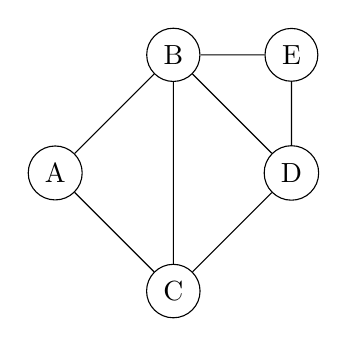
\begin{tikzpicture}[scale=1.5]
            % Define vertices
            \node[circle, draw] (A) at (0, 0) {A};
            \node[circle, draw] (B) at (1, 1) {B};
            \node[circle, draw] (C) at (1, -1) {C};
            \node[circle, draw] (D) at (2, 0) {D};
            \node[circle, draw] (E) at (2, 1) {E};

            % Draw edges to form triangles
            \draw (A) -- (B);
            \draw (A) -- (C);
            \draw (B) -- (C); 
            \draw (B) -- (D);
            \draw (C) -- (D);
            \draw (B) -- (E);
            \draw (D) -- (E);
        \end{tikzpicture}
        \caption{Graph with triangles formed between vertices (A, B, C), (B, C, D) and (B, D, E).}
        \label{fig:triangles}
    \end{minipage}%
\end{figure}

These triangles are more than just theoretical constructs.
In social network graphs, for example, they can represent closed friendships or tightly-knit groups, signaling levels of local connectivity in a network.
This, in turn, can reflect greater patterns and structures within a network.
For example, in social media platforms, triangles are used to model relationships between users, where closed triangles indicate strong communities or mutual interests.
A study analyzing the effect of recommender systems on X (formerly Twitter) demonstrated how an increase in closed triangles following the introduction of a ``Who to Follow'' friend-to-friend recommendation algorithm served as evidence of the algorithm's efficacy \cite{su_effect_2016}.

Additionally, triangles can be used to understand relationships within biological networks.
For example, a study on yeast protein interaction networks used analysis of triangles to find transitive relationships between genes and proteins \cite{ye_commensurate_2005}.
The researchers constructed graphs called ``genetic congruence networks," connecting genes that shared similar interaction partners.
These networks showed a higher-than-expected occurrence of triangles, indicating a strong correlation between genetic congruence and protein interactions.
This suggests that triangles can capture important structural patterns, such as proteins that function within the same biological pathway or complex.
Like in the case of social network analysis, this example illustrates how triangle metrics are not just useful for theoretical analysis but also for practical applications.

While the utility of triangle-based metrics is well-documented, counting triangles efficiently in large graphs remains computationally challenging.
Direct enumeration methods involve inspecting all possible triples of nodes in the graph, a process with a worst-case time complexity of $O(n^3)$ where $n$ is the number of nodes \cite{al_hasan_triangle_2018}.
On smaller networks, this runtime may not pose issues, but unfortunately, for large graphs, especially sparse ones, where the number of edges is much smaller compared to the number of possible edges (as illustrated in Figures \ref{fig:dense_graph} and \ref{fig:sparse_graph}), efficiently counting these triangles poses significant computational challenges.

As graphs grow larger and more complex, direct methods for counting triangles become increasingly time-consuming, making it difficult to handle graphs of practical size in real-world applications.
This issue is particularly relevant in the era of big data, where networks of millions or even billions of nodes and edges are common, and computational efficiency is critical.

\begin{figure}[H]
    \centering
    \begin{minipage}{0.45\textwidth}
        \centering
        % Dense graph
        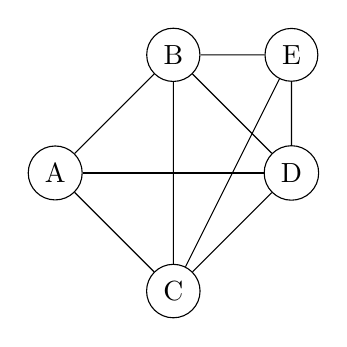
\begin{tikzpicture}[scale=1.5]
            % Define vertices
            \node[circle, draw] (A) at (0, 0) {A};
            \node[circle, draw] (B) at (1, 1) {B};
            \node[circle, draw] (C) at (1, -1) {C};
            \node[circle, draw] (D) at (2, 0) {D};
            \node[circle, draw] (E) at (2, 1) {E};
            % Draw edges to form a dense graph
            \draw (A) -- (B);
            \draw (A) -- (C);
            \draw (A) -- (D);
            \draw (B) -- (C);
            \draw (B) -- (D);
            \draw (B) -- (E);
            \draw (C) -- (D);
            \draw (C) -- (E);
            \draw (D) -- (E);
        \end{tikzpicture}
        \caption{Dense Graph with many edges relative to the number of nodes.}
        \label{fig:dense_graph}
    \end{minipage}%
    \hspace{0.5cm}
    \begin{minipage}{0.45\textwidth}
        \centering
        % Sparse graph
        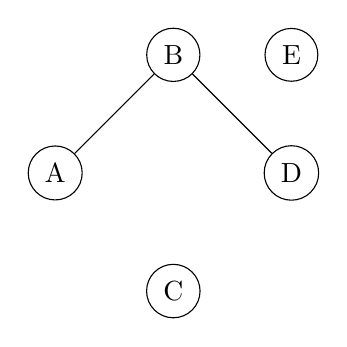
\begin{tikzpicture}[scale=1.5]
            % Define vertices
            \node[circle, draw] (A) at (0, 0) {A};
            \node[circle, draw] (B) at (1, 1) {B};
            \node[circle, draw] (C) at (1, -1) {C};
            \node[circle, draw] (D) at (2, 0) {D};
            \node[circle, draw] (E) at (2, 1) {E};
            % Draw edges to form a sparse graph
            \draw (A) -- (B);
            \draw (B) -- (D);
        \end{tikzpicture}
        \caption{Sparse Graph with few edges relative to the number of nodes.}
        \label{fig:sparse_graph}
    \end{minipage}
\end{figure}

To address these challenges, researchers have developed a variety of approaches to count triangles efficiently.
Some deterministic methods outlined in more detail in the background section of this proposal decrease the time it takes to compute global triangle counts \cite{strassen_gaussian_1969}.
However, these methods still face scalability issues.
As a result, randomized algorithms \cite{tsourakakis_doulion_2009, seshadhri_triadic_2013, tsourakakis_fast_2008} have emerged as a promising alternative.
By leveraging probabilistic techniques, these algorithms provide approximate triangle counts with significant reductions in runtime while maintaining a high degree of accuracy.

Thus, this thesis aims to use randomized algorithms to find new, fast, accurate ways to estimate triangle counts that can be used in real-world applications.

\newpage

\section{Notation}

\begin{table}[ht]
    \centering
    \caption{List of notation used.}
    \begin{tabular}{ll}
        \toprule
        \textbf{Symbol} & \textbf{Description} \\
        \midrule
        $G(V, E)$       & Graph with $V$ vertices and $E$ edges. \\
        $n = |V|$       & Number of vertices in graph $G$. \\
        $m = |E|$       & Number of edges in graph $G$. \\
        $A$             & The adjacency matrix for the graph $G$. \\
        $\Delta_i$      & Number of triangles node $i$ participates in. \\
        $\Delta$        & Total number of triangles in $G$. \\
        $d_i$           & Degree of node $i$. \\
        \bottomrule
    \end{tabular}
    \label{tab:notation}
\end{table}

\newpage

\section{Background}

\subsection{Types of Graphs}

In graph theory, graphs are classified as either directed or undirected.  
An \emph{undirected graph} is one in which edges have no specific direction, so the relationship between connected nodes is mutual: If $u$ connects to $v$, then $v$ connects to $u$.  
In contrast, a \emph{directed graph}, or digraph, has edges with a defined direction—$u$ may point to $v$ without $v$ pointing to $u$.  
This directional property is particularly relevant when calculating triangle counts, as a triangle in a directed graph can follow a specific directional sequence.  
In this discussion, we generally refer to undirected graphs unless otherwise specified, although the methods described can be extended to directed graphs as well.

\subsection{Graph Motifs}

Graph motifs are subgraphs that occur frequently within a larger graph and carry significant structural information.
One such motif is the \emph{clique}, a subset of vertices such that every pair of vertices is connected by an edge.
Triangles, for example, are a clique, as they consist of 3 mutually-connected nodes.
Another common example of a clique is the \emph{4-clique}, denoted as \( K_4 \), which consists of four vertices with edges connecting each pair of vertices.

Formally, we define a 4-clique, \( K_4 \), as the complete graph on four vertices, meaning every pair of vertices is connected by an edge. The set of vertices \( V \) and edges \( E \) for \( K_4 \) are given by:
\[
K_4 = (V, E)
\]
where  
\[
V = \{ v_1, v_2, v_3, v_4 \}, \quad
E = \{ (v_i, v_j) \mid 1 \leq i < j \leq 4 \}.
\]

Figure~\ref{fig:k4} illustrates the structure of \( K_4 \), where each vertex is connected to every other vertex, representing the maximal level of connectivity between four vertices.

\begin{figure}[H]
    \centering
    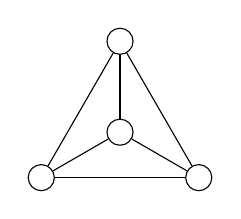
\begin{tikzpicture}[scale=1, every node/.style={circle, draw}]
        % Define the four vertices of K_4
        \node (A) at (0,0) {};
        \node (B) at (2,0) {};
        \node (C) at (1,1.732) {};  % sqrt(3) ≈ 1.732 for equilateral triangle
        \node (D) at (1,0.577) {};  % Center vertex

        % Draw edges to form a complete graph K_4
        \draw (A) -- (B);
        \draw (A) -- (C);
        \draw (A) -- (D);
        \draw (B) -- (C);
        \draw (B) -- (D);
        \draw (C) -- (D);
    \end{tikzpicture}
    \caption{The complete graph \( K_4 \) on four vertices.}
    \label{fig:k4}
\end{figure}

\subsection{Methods for Triangle Counting}

Triangle counting can be approached in a variety of ways, each with its own advantages and disadvantages. 
One of the simplest methods is the brute force technique, where all distinct sets of three vertices ${u, v, w}$ are enumerated and checked for the existence of a triangle.
This involves examining every possible combination of vertices in the graph and testing whether all three edges $(u, v)$, $(v, w)$, and $(w, u)$ exist. 

Assuming optimal conditions with edges stored in a hash table, where edge retrieval takes $O(1)$ time, the time complexity of this brute force approach is $\Theta(n^3)$. 
This complexity stems from the fact that ${n \choose k} = \Theta(n^k)$, and thus, ${n \choose 3} = \Theta(n^3)$ \cite{al_hasan_triangle_2018}. 

While this method is straightforward, it is inefficient for large graphs due to its high computational cost.
Additionally, this method is no more efficient on sparse graphs (those with relatively few edges compared to the maximum number of edges possible) than on dense ones, which is another area for improvement.
Thus, researchers have turned to alternative triangle counting and estimation methods.

\subsubsection{Sampling Methods}

One of the most effective ways to estimate triangle counts in large, sparse graphs is through sampling methods.
These methods rely on randomly selecting edges or vertices and then inspecting their local neighborhoods for the presence of triangles.
Sampling-based techniques are particularly useful in scenarios where calculating the exact triangle count is computationally expensive or unnecessary.

Additionally, sampling algorithms often provide tunable accuracy, allowing for a trade-off between precision and performance, making them ideal for processing large-scale networks.

\subsubsubsection{Edge Sampling}

In edge sampling, we randomly sample a subset of edges from the graph, count the number of triangles in the subgraph, and scale up to reach our estimate.

One key edge sampling algorithm is Doulion \cite{tsourakakis_doulion_2009}, in which each edge in our graph $G$ is sampled with probability $p$.
As all triangles consist of three edges, this means that all triangles in $G$ have probability $p^3$ of being counted.
Thus, the number of triangles counted is scaled by $\frac{1}{p^3}$ to achieve a final estimate.

Other algorithms extend this even further.
For example, a parallel implementation of Doulion \cite{arifuzzaman_parallel_2012}, where each processor independently sparsifies its assigned partition of the graph, can improve accuracy.

In all of these algorithms though, the key piece of their efficiency and efficacy is the sampling of edges to get a good picture of the graph's structure without counting every triangle individually.

\subsubsubsection{Wedge Sampling}

Wedge sampling \cite{seshadhri_triadic_2013} focuses on estimating wedges—triplets of nodes that form two edges but not necessarily a triangle.
A wedge is defined by three vertices $(u, v, w)$ where $u$ is adjacent to both $v$ and $w$, but $v$ and $w$ may or may not be adjacent (see Figure~\ref{fig:wedge_diagram}).

\begin{figure}[H]
    \centering
    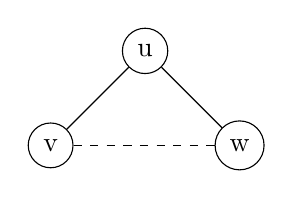
\begin{tikzpicture}[scale = 1.2]
        % Nodes
        \node[circle, draw] (u) at (0,1) {u};
        \node[circle, draw] (v) at (-1,0) {v};
        \node[circle, draw] (w) at (1,0) {w};

        % Edges
        \draw[-] (u) -- (v);
        \draw[-] (u) -- (w);

        % Dashed line to indicate possible or absent connection
        \draw[dashed] (v) -- (w);
    \end{tikzpicture}
    \caption{Wedge formed by vertices $u$, $v$, and $w$. Nodes $v$ and $w$ may or may not be connected.}
    \label{fig:wedge_diagram}
\end{figure}

First, the algorithm counts the total number of wedges in the graph.
To count these wedges, only one pass over all nodes is required, as at each node, every unique pair of outgoing edges from the node is counted as a single wedge.
Thus, this operation takes $O(m)$ time where $m$ is the number of edges in $G$.

Once wedges are sampled, the algorithm checks how many of them are closed (i.e., form triangles).
The number of triangles can then be estimated by multiplying the number of total wedges by the fraction of all wedges that were closed in the sample.
Wedge sampling tends to work well in graphs with a large number of high-degree vertices, where it becomes easier to sample many wedges at once, but unlike edge sampling, it cannot be efficiently done using data structures like adjacency matrices or adjacency lists.
Thus, wedge sampling comes with an additional preprocessing step that adds to runtime.

\subsubsection{Linear Algebraic Methods}

Along with sampling, we can employ linear algebraic techniques to increase the speed of our triangle counting.

Graphs can be conveniently represented using adjacency matrices, which, in social network analysis, are typically referred to as \emph{sociomatrices} \cite{beum_method_1950}. 
In these matrices, each row and column represents a node, and edges between nodes are represented as 1s in the corresponding matrix entry.

\begin{figure}[H]
    \centering
    % Create a minipage for the graph
    \begin{minipage}{0.45\textwidth}
        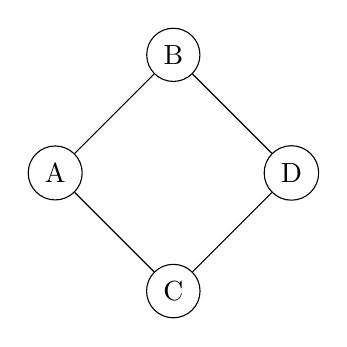
\begin{tikzpicture}[scale=1.5]
            % Define vertices
            \node[circle, draw] (A) at (0, 0) {A};
            \node[circle, draw] (B) at (1, 1) {B};
            \node[circle, draw] (C) at (1, -1) {C};
            \node[circle, draw] (D) at (2, 0) {D};

            % Draw edges
            \draw (A) -- (B);
            \draw (A) -- (C);
            \draw (B) -- (D);
            \draw (C) -- (D);
        \end{tikzpicture}
        \caption{Graph representation of vertices A, B, C, and D.}
    \end{minipage}%
    \hfill
    % Create a minipage for the adjacency matrix
    \begin{minipage}{0.45\textwidth}
        \[
        A =
        \begin{bmatrix}
        0 & 1 & 1 & 0 \\
        1 & 0 & 0 & 1 \\
        1 & 0 & 0 & 1 \\
        0 & 1 & 1 & 0 \\
        \end{bmatrix}
        \]
        \caption{Adjacency matrix corresponding to the graph.}
    \end{minipage}
\end{figure}

By using these adjacency matrices and leveraging linear algebra techniques, we can calculate triangle counts more efficiently. 
One simple method using the adjacency matrix is to use the following formula where $A$ is the adjacency matrix corresponding to the graph $G$ and $\Delta$ is the global triangle count in $G$:

\[
\Delta = \frac{1}{6} \mathrm{trace}(A^3)
\]

This formula is derived from the fact that the diagonal elements of $A^3$ count the number of length-three paths (i.e. triangles) that each vertex participates in.
Each triangle can be formed from six of these length-three paths, as each triangle can be drawn starting at any of its three nodes and moving either clockwise or counter-clockwise, as illustrated in Figure~\ref{fig:triangle-traversal}.
Thus, the trace of $A^3$ is divided by six to scale down to the global triangle count.

\begin{figure}[H]
    \centering
    % First triangle
    \begin{subfigure}{0.15\textwidth}
        \centering
        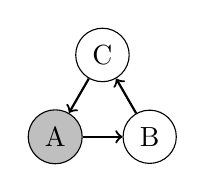
\begin{tikzpicture}[scale=1.2]
            % Define vertices
            \node[circle, draw, fill=gray!50] (A) at (0,0) {A};
            \node[circle, draw] (B) at (1,0) {B};
            \node[circle, draw] (C) at (0.5,0.866) {C};

            % Draw edges with arrows
            \draw[thick, ->] (A) -- (B);
            \draw[thick, ->] (B) -- (C);
            \draw[thick, ->] (C) -- (A);
        \end{tikzpicture}
    \end{subfigure}
    % Second triangle
    \begin{subfigure}{0.15\textwidth}
        \centering
        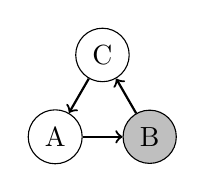
\begin{tikzpicture}[scale=1.2]
            % Define vertices
            \node[circle, draw, fill=gray!50] (B) at (1,0) {B};
            \node[circle, draw] (C) at (0.5,0.866) {C};
            \node[circle, draw] (A) at (0,0) {A};

            % Draw edges with arrows
            \draw[thick, ->] (B) -- (C);
            \draw[thick, ->] (C) -- (A);
            \draw[thick, ->] (A) -- (B);
        \end{tikzpicture}
    \end{subfigure}
    % Third triangle
    \begin{subfigure}{0.15\textwidth}
        \centering
        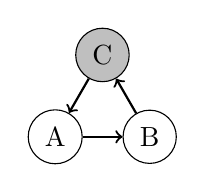
\begin{tikzpicture}[scale=1.2]
            % Define vertices
            \node[circle, draw, fill=gray!50] (C) at (0.5,0.866) {C};
            \node[circle, draw] (A) at (0,0) {A};
            \node[circle, draw] (B) at (1,0) {B};

            % Draw edges with arrows
            \draw[thick, ->] (C) -- (A);
            \draw[thick, ->] (A) -- (B);
            \draw[thick, ->] (B) -- (C);
        \end{tikzpicture}
    \end{subfigure}
    % Fourth triangle
    \begin{subfigure}{0.15\textwidth}
        \centering
        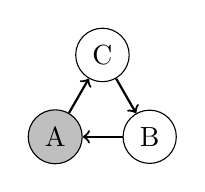
\begin{tikzpicture}[scale=1.2]
            % Define vertices
            \node[circle, draw, fill=gray!50] (A) at (0,0) {A};
            \node[circle, draw] (C) at (0.5,0.866) {C};
            \node[circle, draw] (B) at (1,0) {B};

            % Draw edges with arrows
            \draw[thick, ->] (A) -- (C);
            \draw[thick, ->] (C) -- (B);
            \draw[thick, ->] (B) -- (A);
        \end{tikzpicture}
    \end{subfigure}
    % Fifth triangle
    \begin{subfigure}{0.15\textwidth}
        \centering
        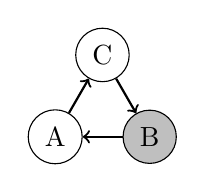
\begin{tikzpicture}[scale=1.2]
            % Define vertices
            \node[circle, draw, fill=gray!50] (B) at (1,0) {B};
            \node[circle, draw] (A) at (0,0) {A};
            \node[circle, draw] (C) at (0.5,0.866) {C};

            % Draw edges with arrows
            \draw[thick, ->] (B) -- (A);
            \draw[thick, ->] (A) -- (C);
            \draw[thick, ->] (C) -- (B);
        \end{tikzpicture}
    \end{subfigure}
    % Sixth triangle
    \begin{subfigure}{0.15\textwidth}
        \centering
        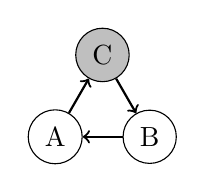
\begin{tikzpicture}[scale=1.2]
            % Define vertices
            \node[circle, draw, fill=gray!50] (C) at (0.5,0.866) {C};
            \node[circle, draw] (B) at (1,0) {B};
            \node[circle, draw] (A) at (0,0) {A};

            % Draw edges with arrows
            \draw[thick, ->] (C) -- (B);
            \draw[thick, ->] (B) -- (A);
            \draw[thick, ->] (A) -- (C);
        \end{tikzpicture}
    \end{subfigure}
    \caption{Six different ways to arrive at a length-three path in a triangle.}
    \label{fig:triangle-traversal}
\end{figure}

To compute $A^3$, we first need to calculate $A^2$ (which takes $O(n^3)$ for an $n \times n$ matrix, $n$ thus also being the number of nodes in our graph $G$) and then multiply $A^2$ by $A$ (also $O(n^3)$).
Thus, the total complexity for computing $A^3$ is $O(n^3)$.
After computing $A^3$, calculating the trace takes $O(n)$, as we need to iterate over the $n$ diagonal elements.
Thus, the overall runtime complexity for the operation is $O(n^3)$.
While this is not a direct improvement over the runtime of the naive algorithm, this strategy forms the basis of many faster methods.

\subsubsubsection{Strassen's Algorithm}

This runtime analysis above assumes that matrix multiplication is performed using the standard algorithm.
However, more sophisticated techniques, such as Strassen's algorithm \cite{strassen_gaussian_1969}, can reduce matrix multiplication time.
In this algorithm, that is used on large, square matrices, such as undirected sociomatrices, each matrix is divided into smaller submatrices on which a series additions and multiplications are performed.

Specifically, Strassen's algorithm reduces the complexity of multiplying two $n \times n$ matrices to approximately $O(n^{\log_2 7})$, which is about $O(n^{2.81})$.
Computing $A^2$ using Strassen's algorithm will take $O(n^{\log_2 7})$.
Then, multiplying $A^2$ by $A$ again takes $O(n^{\log_2 7})$.
Therefore, the total complexity for computing $A^3$ with Strassen's algorithm is $O(n^{\log_2 7}) + O(n^{\log_2 7}) = O(n^{\log_2 7})$, or roughly $O(n^{2.81})$.

To contextualize this, on a $2 \times 2$ matrix, the $n^3$ multiplications required for the naive method would mean we would complete $2^3 = 8$ multiplications.
With Strassen's method and its $n^{\log_2 7}$ multiplications, there would instead only be $2^{\log_2 7} = 7$ multiplications computed.
On larger matrices, this leads to a significant speedup.

There are matrix multiplication algorithms that are even faster, such as one with a $O(n^{2.371552})$ runtime, but this algorithm relies on the use of extremely large constants and is thus rarely used in real-world applications \cite{williams_new_2023}.

\subsubsubsection{EigenTriangle Algorithm}

Another significant approach in triangle counting is the use of spectral methods.
One such method is the EigenTriangle algorithm \cite{tsourakakis_fast_2008}, which estimates the triangle count $\Delta$ by considering the spectral decomposition of the adjacency matrix $A$.

The EigenTriangle algorithm is based on the observation that the number of triangles in a graph is closely related to the spectrum of its adjacency matrix.
In particular, the adjacency matrix $A$ is decomposed as:

\[
A = U \Lambda U^T,
\]

where $U$ is a matrix whose columns are the eigenvectors of $A$, and $\Lambda$ is a diagonal matrix containing the corresponding eigenvalues.

Once the decomposition is performed, the number of triangles can be computed exactly using $\Delta = \frac{1}{6} \sum_{i=1}^{n} \lambda_i^3$, and can be estimated using:

\[
\Delta \approx \frac{1}{6} \sum_{i=1}^{k} \lambda_i^3,
\]

where $\lambda_i$ are the $k$ eigenvalues of largest magnitude of the adjacency matrix $A$.
The runtime of EigenTriangle is dominated by the cost of approximating the top $k$ eigenvalues and eigenvectors of $A$, which, using the Lanszos method \cite{cullum_lanczos_2002}, can be done in roughly $O(k m)$ time, where $m$ is the number of edges and $k$ is typically much smaller than the number of nodes $n$.
This is a significant improvement over the runtimes of direct methods.

Specifically, for the direct method in which was compute the trace of $A^3$, we know ${trace}(A^3) = \sum_{i = 1}^{n} \lambda_i(A^3) = \sum_{i = 1}^{n} \lambda_i^3$.
Thus, we see that EigenTriangle approximates ${trace}(A^3)$.
Given this, it makes sense that this runtime is a substantial improvement over the complexity of computing $\mathrm{trace}(A^3)$ directly.

\subsubsubsection{TraceTriangle Algorithm}

The TraceTriangle algorithm \cite{avron_counting_2010} is a randomized algorithm designed for efficient triangle estimation in large graphs.
It leverages trace-based techniques, which compute the trace of matrix powers to approximate the number of triangles.
Specifically, the algorithm relies on the previously mentioned property: $\Delta = \frac{1}{6} \mathrm{trace}(A^3)$, where $A$ is the adjacency matrix of the graph and $\Delta$ is the number of triangles.
However, rather than computing the full matrix multiplication $A^3$, which is computationally expensive for large graphs, the TraceTriangle algorithm uses a randomized approach to approximate this trace, significantly reducing computation time.

This randomized approach is based on Hutchinson's method \cite{hutchinson_stochastic_1990}, which is a technique for estimating the trace of a matrix by randomly sampling vectors.
In this case, this significantly reduces computation time by approximating $\mathrm{trace}(A^3)$ through randomized sampling rather than explicit computation.

The TraceTriangle algorithm is a sampling algorithm, and thus, it's runtime depends on the desired accuracy of output, as more or fewer samples can be taken depending on the application.
Generally though, experiments demonstrate that typically $O(log^2|n|)$, where $n$ is the number of vertices in $G$, samples are required to get good approximations on real-world graphs, and regardless of application, the runtime for taking each sample is $O(|m|)$, where $m$ is the number of edges in $G$.

Comparing TraceTriangle to the EigenTriangle algorithm, TraceTriangle achieves higher accuracy across multiple types of graphs \cite{avron_counting_2010}.
Despite this accuracy advantage, EigenTriangle tends to run more quickly than TraceTriangle on large graphs.
That said, one advantage of TraceTriangle is its potential for parallelization.
This allows TraceTriangle to scale effectively with the size of the graph, ultimately reducing the speed advantage of EigenTriangle in larger computations.

\subsection{General Algorithmic Strategies}

Beyond specific algorithms for triangle counting, various general techniques from theoretical computer science have been adapted for this problem, particularly in designing faster algorithms.

\subsubsection{Variance Reduction}
\label{sec:variance-reduction-background}

Variance reduction \cite{prescott_monte_1965} is another general technique that can be applied to triangle estimation, improving accuracy without increasing the number of samples needed.

Variance reduction methods aim to reduce the spread (or variance) of estimations, leading to more reliable results even with fewer samples.
This is particularly important in large-scale graphs, where taking a high number of samples may be computationally infeasible.

In terms of triangle counting, this method can be applied by finding a fast way of estimating the global triangle count, and then using sampling to estimate the error on that count.
Specifically, we can begin by finding a relationship between the degree of nodes and the number of triangles they are involved in.
This can be done by plotting nodes' degrees ($d_i$) versus triangle counts $(\Delta_i)$ on a log-log plot, finding a line of best fit, and then exponentiating as follows:

\[
\log(\Delta_i) \approx \alpha \cdot \log(d_i) + \beta
\]
\[
\Delta_i \approx d_i^\alpha \cdot e^\beta = m_i.
\]

Now, using this equation, we can estimate the overall triangle count $M$ by applying this line of best fit relationship to all nodes in the graph:

\[
M = \sum_{i = 1}^{n} m_i.
\]

Next, we sample our graph to get $s$ nodes, with $s$ being our sample size. For each of these $s$ sampled nodes, we count the number of triangles they are involved in (written $\Delta_i$) and find the difference between those actual triangle counts and their estimated triangle counts using the line of best fit relationship. We then take the sum of these errors and scale them up to estimate the error on our global triangle count (written $E$). Mathematically, this can be expressed as follows:

\[
E = \left( \sum_{i = 1}^{s} \Delta_i - m_i \right) \cdot \frac{n}{s}.
\]

Lastly, we take the sum of our estimate and our error, and divide this sum by three to avoid triple-counting triangles, as each triangle has three nodes it is involved in:

\[
\Delta \approx \frac{M + E}{3}.
\]

Thus, by applying this variance reduction technique, we arrive at an estimate for the triangle count $\Delta$.

\subsubsection{Importance Sampling}
\label{sec:importance-sampling-background}

One example of a variance reduction method is importance sampling.
When estimating a metric relating to a large population using uniform sampling, where all edges/nodes/wedges/etc. are sampled with the same probability, often a very large number of samples is required to ensure a good relative approximation \cite{lovasz_large_2012}.
This is because uniform sampling does not prioritize areas of the graph that may have a disproportionately large impact on the estimate.
Consequently, the computational cost can be high for achieving a desired accuracy level in many cases.

When using importance sampling \cite{motwani_randomized_1995}, the process is improved by sampling higher-interest nodes with higher probability, focusing computational effort on the most ``important" parts of a graph.
The key idea behind importance sampling is to bias the sampling distribution towards more informative areas of the graph.
For instance, in a graph where certain nodes are highly connected or play a critical role in the overall structure, importance sampling would prioritize these nodes to reduce the variance of the estimates.

Importance sampling can also be applied to triangle counts.
For example, we can prioritize high-degree nodes as the most ``important.''
The weight of this importance is decided by some power $\alpha$ greater than 1 (which is equivalent to uniform sampling).
This $\alpha$ can be tuned to indicate different strengths of relationships between the degree and triangle counts of nodes. 

To get the optimal value for $\alpha$, we can plot nodes' degrees versus triangle count as described in section \ref{sec:variance-reduction-background} and use the value of the slope ($\alpha$) obtained when calculating the line of best fit of this plot.

Once $\alpha$ has been selected, we use it to ascribe each node a probability $p_i$ to each node based in its degree $d_i$:

\[
D = \sum_{i = 1}^{n} d_i^\alpha
\]
\[
p_i = \frac{d_i^\alpha}{D}.
\]

Next, we sample $s$ nodes based on their probabilities $p_i$.
For example if $p_1 = 0.01$ and $p_2 = 0.1$, we are 10 times more likely to sample node 2 than node 1.

Next, for each sampled node we count the number of triangles it is a part of, and then scale that count by $\frac{1}{s \cdot p_i}$.
The sum of all these counts, scaled down by three (as to avoid triple-counting triangles), is our estimate for the global triangle count $\Delta$.

\subsubsection{Learning-Augmented Algorithms}

A learning-augmented algorithm \cite{roughgarden_algorithms_2020} is an algorithm that uses a prediction to boost its performance.
Whereas most algorithms take only the problem their input, learning-augmented algorithms also accept an extra piece of information—usually a prediction about some part of the solution.
The algorithm then uses this prediction to run faster or produce better results.

An example of a learning-augmented algorithm is its use in the maximum weight matching problem.
The maximum weight matching problem \cite{duan_linear-time_2014} is the problem of finding a matching in which the sum of weights is maximized in a weighted graph.
The typical solution for this problem, the Hungarian algorithm, runs in $O(m\sqrt{n})$ time.

When a learning-augmented approach \cite{dinitz_faster_2021} is applied however, where machine-learned predictions are used to ``warm-start" the algorithm, that runtime is significantly reduced when the predictions are accurate.
When the predictions are inaccurate, the runtime is simply the same as in the Hungarian algorithm.

This technique can be applied to triangle counting too.
For example, Tonic \cite{boldrin_fast_2024}, a learning-augmented algorithm for counting triangles in graph streams, leverages predictions about edge ``heaviness" (i.e., the number of triangles they are involved in) to improve the accuracy and speed of triangle counting.
Tonic combines these predictions with sampling methods to keep track of the most relevant edges.
This allows the algorithm to focus on the edges that are most likely to contribute to the triangle count.

Notably, Tonic provides unbiased estimates of triangle counts regardless of the accuracy of the predictor.
However, when the predictor provides useful information on heavy edges, the algorithm produces estimates with reduced variance compared to state-of-the-art alternatives.

In general, this method can be highly effective, as accurate predictions can significantly enhance algorithms' efficiency or result quality.

\newpage

\section{Methods}

To evaluate different triangle count estimation methods, I implemented them in Python and compared their accuracies, runtimes, and sample sizes on a diverse set of networks.
The primary methods implemented were uniform sampling, importance sampling, a variance reduction method, and a hybrid method that combines elements of these approaches. 

The implemented methods were applied to both synthetic and real-world networks sourced from the \href{https://snap.stanford.edu/index.html}{Stanford Network Analysis Platform (SNAP) library}.
These networks span a range of sizes, densities, and structural properties to ensure robust comparisons.

\subsection{Implementation}

Algorithms were implemented in Python using NetworkX and SNAP, and experiments were run on consistent hardware, with multiple trials to ensure reliable comparisons.

\subsection{Datasets}

The datasets used in this study include both synthetic networks and real-world graphs from the SNAP library, covering various domains such as social networks, collaboration networks, and web graphs.
Specifically, methods were evaluated on these three networks:

\begin{itemize}
    \item \href{https://snap.stanford.edu/data/ego-Facebook.html}{Social Network (Facebook)}: Social circles (or `friends lists') are represented in this graph, where each user is a node, and each edge is a friendship between users.
    \item \href{https://snap.stanford.edu/data/ca-GrQc.html}{Collaboration Network}: This graph represents a network of co-authorships from the General Relativity and Quantum Cosmology collaboration network, where nodes represent authors and edges indicate co-authored papers.
    \item \href{https://snap.stanford.edu/data/wikipedia-article-networks.html}{Wikipedia Article Network}: This graph represents a network of Wikipedia articles relating to crocodiles, where nodes represent articles and edges represent links between them.
\end{itemize}

A synthetic network was also generated using the \href{https://networkx.org/}{NetworkX library}.
Specifically, the library was used to create a Barabási–Albert \cite{albert_statistical_2002} graph.
Barabási–Albert graphs model preferential attachment, exhibiting power-law degree distributions, making them interesting graphs when using degree as a predictor for other graph features.

To assess accuracy, ground-truth triangle counts were computed using exact algorithms and compared against the approximate counts produced by each estimation method.
The evaluation metrics included accuracy, runtime efficiency, and the sample size required to achieve a specified error margin.
By examining performance across different graph characteristics, the study identifies the strengths and weaknesses of each method in diverse scenarios.

\subsection{Sampling Methods Evaluated}

\subsubsubsection{Uniform Sampling:}

This baseline method involves randomly sampling edges or nodes and scaling up the observed triangle counts proportionally.
While simple, uniform sampling often struggle in graphs with skewed degree distributions.

Code for this method is given below, where $A$ is the adjacency matrix of our graph $G$ and $s$ is the number of nodes of $G$ being sampled.

\begin{lstlisting}[language=Python]
import numpy as np
import random

def gen_s_ints(s, n):
    choice_arr = sorted(random.choices(range(n), k=s))
    return choice_arr

def estimate_uniformly_per_node_method(A, s):
    n = len(A)
    sampled_nodes = gen_s_ints(s, n)

    triangle_count = 0
    for i in sampled_nodes:
        triangle_count += count_node_triangles(A, i)

    return triangle_count * (n / s) // 3

\end{lstlisting}

\textbf{Importance Sampling:}

In this method, we attempt to prioritize the sampling of nodes that are likely to form more triangles.
This is done by sampling proportionally to the degree of nodes.
This method aims for higher accuracy with fewer samples.


As written in section \ref{sec:importance-sampling-background}, in importance sampling, after we select a value $\alpha$ to indicate the strength of the relationship between the degree and triangle count of nodes, we can use this value $\alpha$ to ascribe each node a probability $p_i$ to each node based in its degree $d_i$:

\[
D = \sum_{i = 1}^{n} d_i^\alpha
\]
\[
p_i = \frac{d_i^\alpha}{D}.
\]

We can then sample each node $n_i$ with probability $p_i$.
The code for this sampling and estimation process is given below where, like before $A$ is the adjacency matrix of $G$ and $s$ is our sample size.
We also introduce the parameter $\alpha$, which in the code snippet, is represented by the variable ``power''.

\begin{lstlisting}[language=Python]
def sample_by_degree(A, n, s, power):
    degrees = np.sum(A, axis=1)
    degrees_to_power = np.power(degrees, power)

    sum_of_degrees_to_power = np.sum(degrees_to_power)
    probabilities = degrees_to_power / sum_of_degrees_to_power

    sampled_nodes = random.choices(range(n), weights=probabilities, k=s)

    return probabilities, sampled_nodes

def importance_estimate_per_node_method(A, s, power):
    n = len(A)
    probabilities, sampled_nodes = sample_by_degree(A, n, s, power)

    estimate = 0
    for i in sampled_nodes:
    triangle_count = count_node_triangles(A, i)
    estimate += triangle_count * (1 / (s * probabilities[i]))

    return estimate // 3
\end{lstlisting}

To select the ideal value for the power ($\alpha$), as described in section \ref{sec:importance-sampling-background}, we plot nodes' degrees verses triangle counts and set $\alpha$ to be the slope of this plot.

The dataset we will primarily use is the Social Network (Facebook) dataset.

\begin{figure}[H]
    \centering
    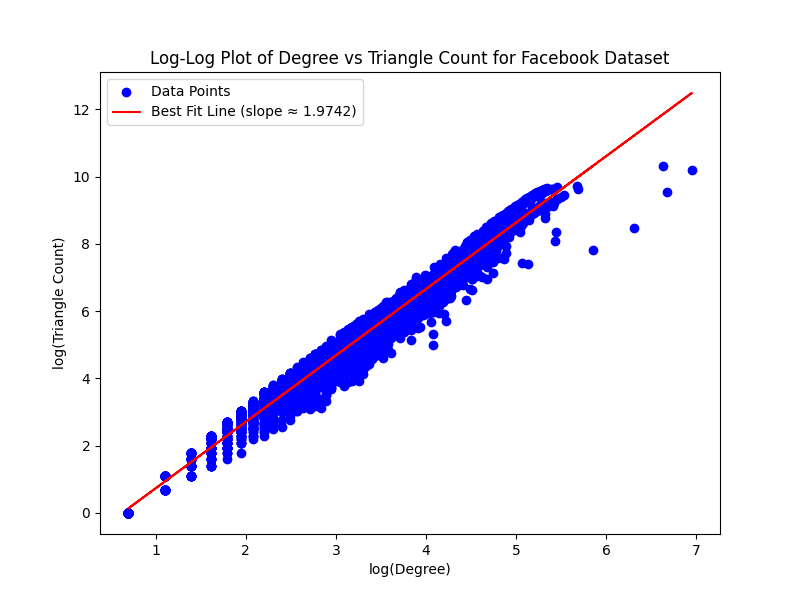
\includegraphics[width=0.8\textwidth]{plots/degree-vs-triangle-count/degree_vs_triangle_count_fb.png}
    \caption{Degree vs. triangle count for the Facebook dataset. The slope $\alpha \approx 1.97$.}
    \label{fig:degree_vs_tri_fb}
\end{figure}

The slope $\alpha$  in figure \ref{fig:degree_vs_tri_fb} is $~ 1.97$.
Below, we give the degree vs triangle count plots for the other three datasets used:

\begin{figure}[H]
    \centering
    \begin{subfigure}[b]{0.31\textwidth}
        \centering
        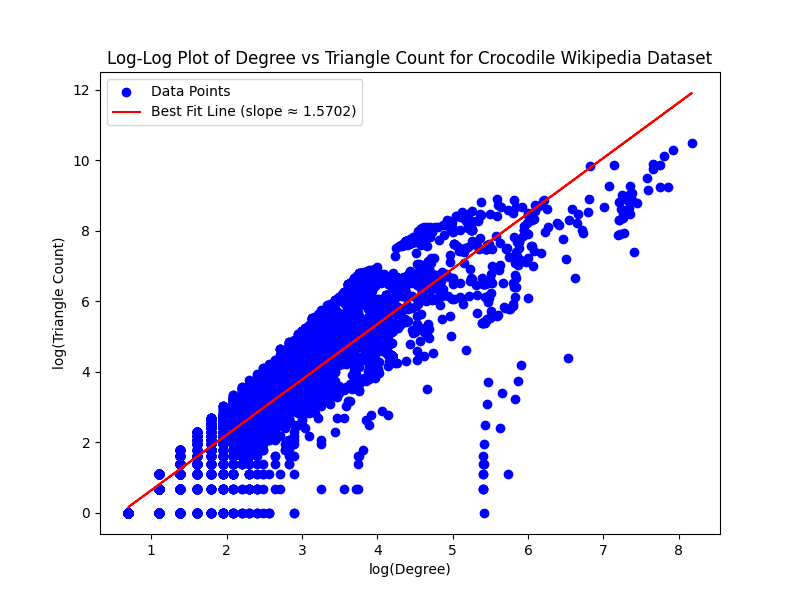
\includegraphics[width=\textwidth]{plots/degree-vs-triangle-count/degree_vs_triangle_count_croc.png}
        \caption{Wikipedia}
        \label{fig:degree_vs_tri_croc}
    \end{subfigure}
    \hfill
    \begin{subfigure}[b]{0.31\textwidth}
        \centering
        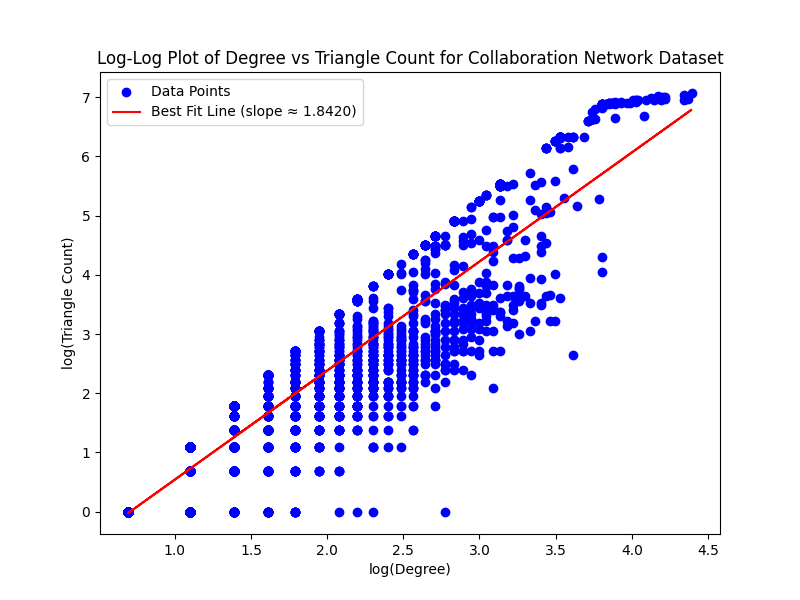
\includegraphics[width=\textwidth]{plots/degree-vs-triangle-count/degree_vs_triangle_count_GrQc.png}
        \caption{Collaboration}
        \label{fig:degree_vs_tri_GrQc}
    \end{subfigure}
    \hfill
    \begin{subfigure}[b]{0.31\textwidth}
        \centering
        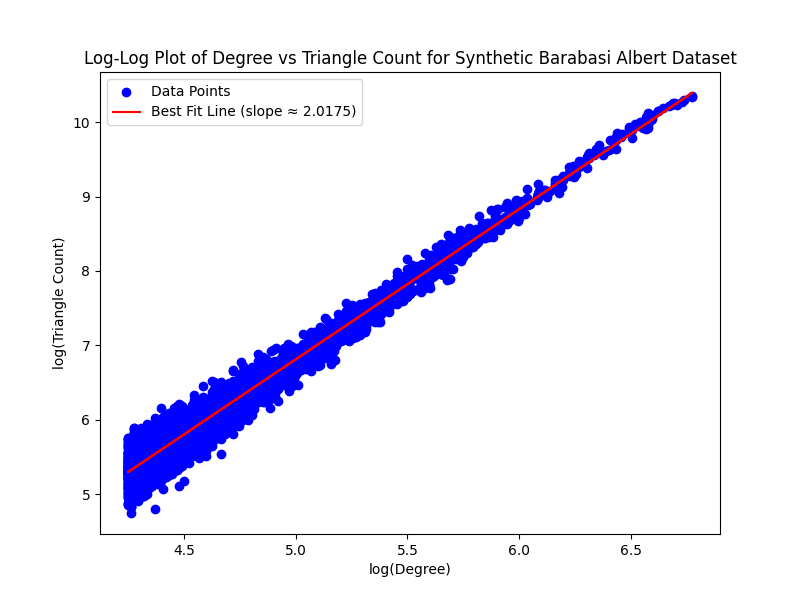
\includegraphics[width=\textwidth]{plots/degree-vs-triangle-count/degree_vs_triangle_count_ba.png}
        \caption{Barabási–Albert}
        \label{fig:degree_vs_tri_ba}
    \end{subfigure}

    \caption{Degree vs. triangle count across datasets. For the Wikipedia dataset $\alpha \approx 1.57$, for the collaboration network $\alpha \approx 1.84$, and for the Barabási–Albert graph $\alpha \approx 2.02$.}
    \label{fig:degree_vs_tri_others}
\end{figure}

Given the spread of $\alpha$ values obtained, we set our default value of $\alpha$ to 2, but also tested values 1 and 1.5 for all datasets.
In addition, for each dataset, run importance sampling was run with the ``optimal'' $\alpha$ found in its scatter plot.

\textbf{Variance Reduction:}
\label{variance-reduction-algo}

Our next method is variance reduction, which aims minimize the variability of our estimates.
The high variance in uniform or importance sampling methods can lead to inaccurate triangle count estimations, particularly in graphs with skewed degree distributions.
To address this, we leverage additional information about the relationship between node degrees and triangle counts.

In many real-world graphs, nodes with higher degrees tend to form more triangles, suggesting a potential correlation between the log of the degree and the log of the triangle count.
Thus, by performing a linear regression in log-log space, we can obtain a line of best fit that estimates triangle counts as a function of node degree, and use that to arrive an an estimate of our triangle count.

However, the number arrived at using our linear regression may either over- or under-count the number of triangles depending on the relationship between degree and triangle count.
Thus, we sample $s$ additional nodes and calculate the difference between their actual triangle counts and those predicted by our line of best fit.
Then, scaling this up, we can combine our predicted triangle count and predicted error to arrive at a final estimate of the triangle count $\Delta$.

The specific math for this method is given in section \ref{sec:variance-reduction-background} and the code for it is given below.

\begin{lstlisting}[language=Python]
def get_line_of_best_fit(A):
    n = len(A)
    degrees = np.sum(A, axis=1)
    triangles = np.zeros(n)

    for i in range(n):
        triangles[i] = count_node_triangles(A, i)

    valid_indices = (degrees > 0) & (triangles > 0)
    filtered_degrees = degrees[valid_indices]
    filtered_triangles = triangles[valid_indices]

    log_degrees = np.log(filtered_degrees)
    log_triangles = np.log(filtered_triangles)

    slope, intercept = np.polyfit(log_degrees, log_triangles, 1)

    return slope, intercept

def estimate_variance_reduction_method(A, s, power):
    n = len(A)
  
    slope, intercept = get_line_of_best_fit(A)
  
    # obtain M from the line of best fit
    degree_array = np.sum(A, axis=1)
    approx_triangles = np.power(degree_array, slope) * np.exp(intercept)
    M = np.sum(approx_triangles)
  
    if s == 0:
        return M // 3
  
    # sample s nodes, and use them to adjust our estimate M
    sampled_nodes = gen_s_ints(s, n)
    sampled_node_triangles = np.array([count_node_triangles(A, i) for i in sampled_nodes])
  
    sampled_m_i_vals = np.array([approx_triangles[i] for i in sampled_nodes])
  
    D = np.sum(sampled_node_triangles - sampled_m_i_vals) * (n/s)
  
    return (M + D) // 3
\end{lstlisting}

\textbf{Hybrid Approach:}

The hybrid approach combines elements from both importance sampling and variance reduction techniques.
It functions by running the variance reduction method as before, but using importance sampling instead of uniform sampling to generate the $s$ nodes used in correcting our triangle count estimate.

The differences between the following code snippet and that in variance reduction begins on line 13.

\begin{lstlisting}[language=Python]
def estimate_importance_variance_reduction_method(A, s, power):
    n = len(A)

    slope, intercept = get_line_of_best_fit(A)

    degree_array = np.sum(A, axis=1)
    approx_triangles = np.power(degree_array, slope) * np.exp(intercept)
    M = np.sum(approx_triangles)

    if s == 0:
        return M // 3

    probabilities, sampled_nodes = sample_by_degree(A, n, s, power)
    sampled_node_probabilities = np.array([probabilities[i] for i in sampled_nodes])
    sampled_node_triangles = np.array([count_node_triangles(A, i) for i in sampled_nodes])

    sampled_m_i_vals = np.array([approx_triangles[i] for i in sampled_nodes])

    D = np.sum((sampled_node_triangles - sampled_m_i_vals) * (1 / (s * sampled_node_probabilities)))

    return (M + D) // 3
\end{lstlisting}

Values for $\alpha$ for this hybrid method were selected the same way they were for importance sampling.

\subsection{Evaluation Metrics}

To assess the performance of the triangle count estimation methods, the following evaluation metrics were measured on real-world and synthetic networks:

\begin{itemize}
\item Accuracy: The difference between the estimated and true triangle counts, calculated as the relative error.
\item Runtime: The computational time required to generate triangle count estimates.
\item Sample size: The number of nodes or edges sampled to produce an estimate.
\item Variance: The variability in triangle count estimates across multiple independent runs of the same method.
\end{itemize}

\subsection{Additional Explorations}

\subsubsection{4-Clique Variant}

To evaluate how well these methods generalize, the code for each algorithm was adapted to count 4-cliques.
To adapt the previous methods to count 4-cliques, we simply replace the \lstinline{count_node_triangles()} method with a \lstinline{count_node_4_cliques()} method, and scale final results by 4 instead of by 3.

To find the optimal values for $\alpha$ like before, we would plot degree versus 4-clique count and calculate a line of best fit.
Likely, the optimal values would be close to 3.
However, in this thesis, I only tested on values of $\alpha$ of 1 and 1.5 as this variant is intended as a preliminary extension to demonstrate feasibility rather than to optimize performance
 More extensive tuning of $\alpha$ and evaluation across a wider range of graphs would be a valuable direction for future work.

\subsubsection{Simulated Method Tests}

In order to learn more about when importance sampling and variance reduction perform best, I ran these algorithms on manually defined triangle-degree relationships.

The methods were tested on two different degree-triangle relationships.
First, I set a variable \lstinline{degrees} to be the degree distribution of a real-world dataset.
I also defined \lstinline{noise} as \lstinline{noise = np.random.normal(0, noise_scale, triangles.shape)}.
This noise is normally distributed with a mean of zero and a standard deviation of \lstinline{noise_scale}, allowing for random fluctuations around the expected triangle and maintaining a symmetric distribution.

The two relationships defined using these degrees and noise values are the \textbf{Uniform noise} and \textbf{multiplicative noise} relationships.
For the first, artificial triangle counts for the degree distributions were set to \lstinline{np.power(degrees, slope) * np.exp(intercept) + noise} where the slope and intercept are the outputs from the \lstinline{get_line_of_best()} function defined in section \ref{variance-reduction-algo}.
Thus, in this relationship, noise does not grow with degree.

For the second relationship, the \textbf{multiplicative noise} relationship, the artificial triangle counts were set to \lstinline{np.power(degrees, slope) * np.exp(intercept) * (1 + noise)} where the slope, intercept, and noise are defined as before.
In this relationship, noise grows as the degree does too, distinguishing this degree-triangle relationship from the former.

These noise models allow us to analyze how different types of randomness impact the performance of variance reduction and importance sampling techniques.

\newpage

\section{Results}

\subsection{Triangle Counting}

\subsubsection{Average Percent Error By Method}

In this section, we present the average percent error of estimating triangle counts for each method.
All of this data comes from the Social Network (Facebook) dataset.

\begin{figure}[H]
    \centering
    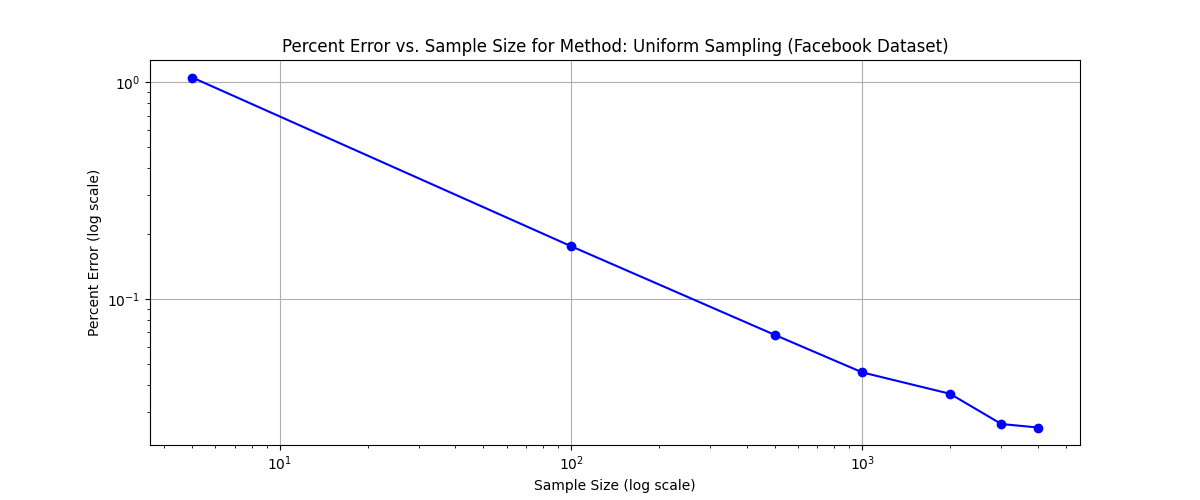
\includegraphics[width=0.8\textwidth]{plots/percent-errors/percent_error_Uniform Sampling.png}
    \caption{Percent Error - Uniform Sampling. Percent error decreases as sample size increases.}
    \label{fig:percent_error_uniform}
\end{figure}

\begin{figure}[H]
    \centering
    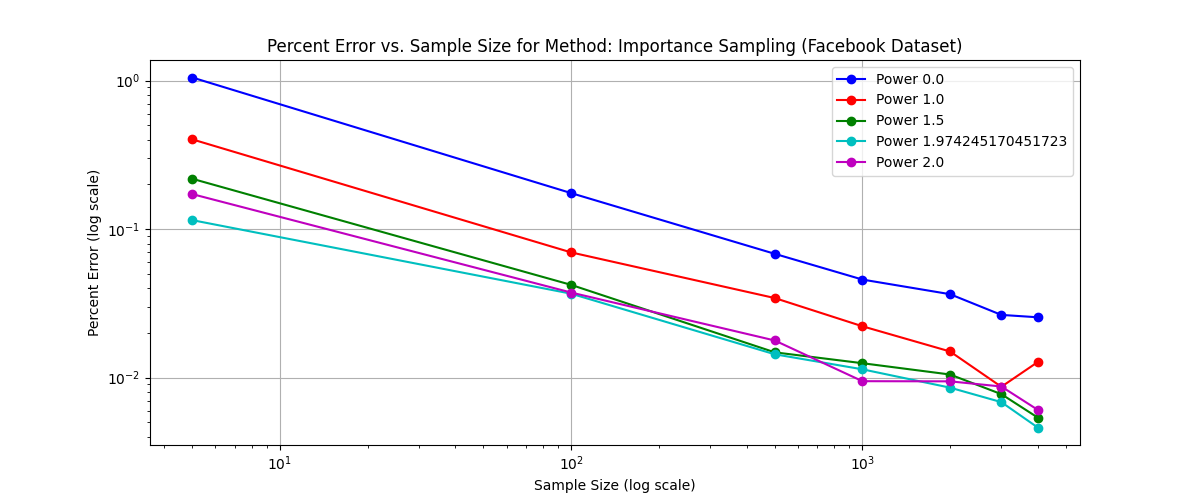
\includegraphics[width=0.8\textwidth]{plots/percent-errors/percent_error_Importance Sampling.png}
    \caption{Percent Error - Importance Sampling. Percent error decreases as sample size increases. Powers closest to ~1.97 perform best.}
    \label{fig:percent_error_importance}
\end{figure}

\begin{figure}[H]
    \centering
    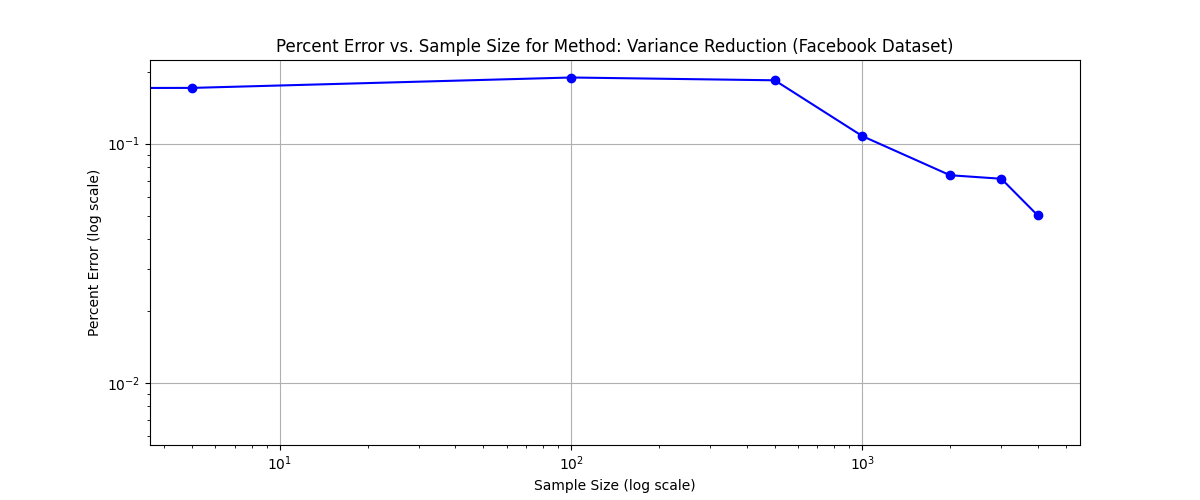
\includegraphics[width=0.8\textwidth]{plots/percent-errors/percent_error_Variance Reduction.png}
    \caption{Percent Error - Variance Reduction. Percent error decreases as sample size increases once the sample size is large enough.}
    \label{fig:percent_error_variance}
\end{figure}

\begin{figure}[H]
    \centering
    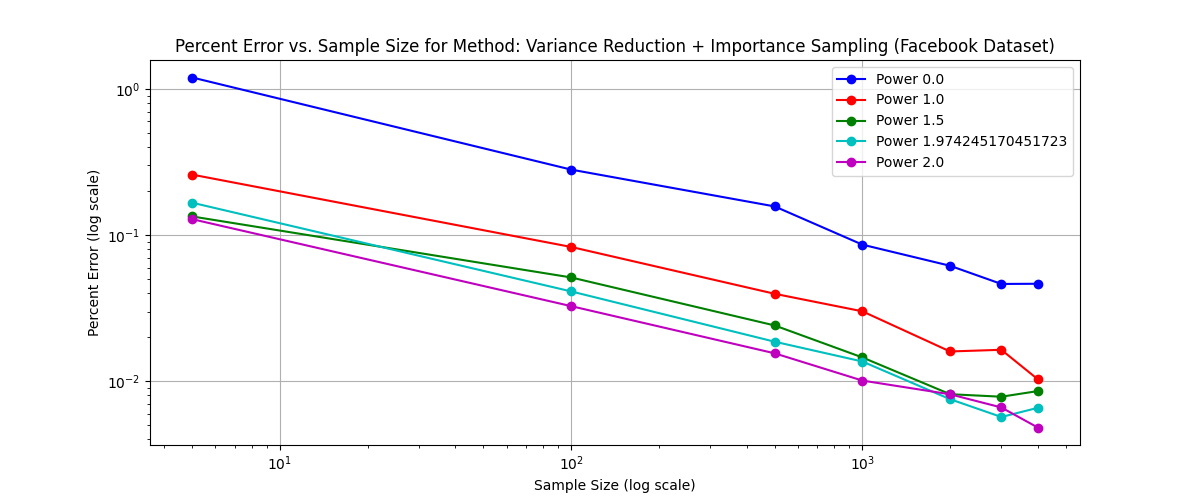
\includegraphics[width=0.8\textwidth]{plots/percent-errors/percent_error_Variance Reduction + Importance Sampling.png}
    \caption{Percent Error - Variance Reduction + Importance Sampling. Percent error decreases as sample size increases. Powers closest to ~1.97 perform best.}
    \label{fig:percent_error_variance_importance}
\end{figure}

\subsubsection{Average Duration (Runtime) By Method}

In this section, we display the average duration of estimating triangle counts for each method.
All of this data comes from the Social Network (Facebook) dataset.

\begin{figure}[H]
    \centering
    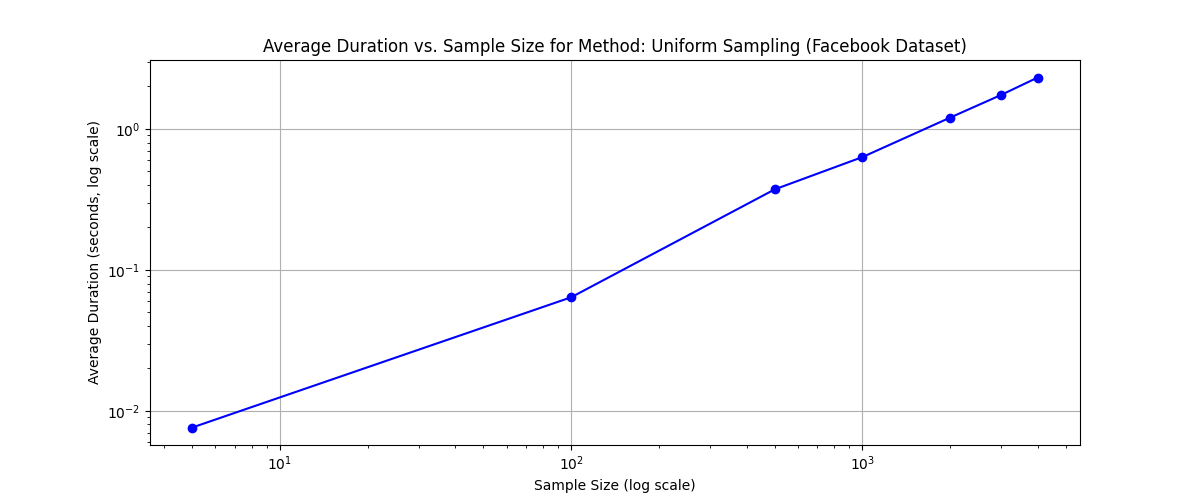
\includegraphics[width=0.8\textwidth]{plots/durations/avg_duration_Uniform Sampling.png}
    \caption{Average Duration - Uniform Sampling. Runtime increases with sample size.}
    \label{fig:avg_duration_uniform}
\end{figure}

\begin{figure}[H]
    \centering
    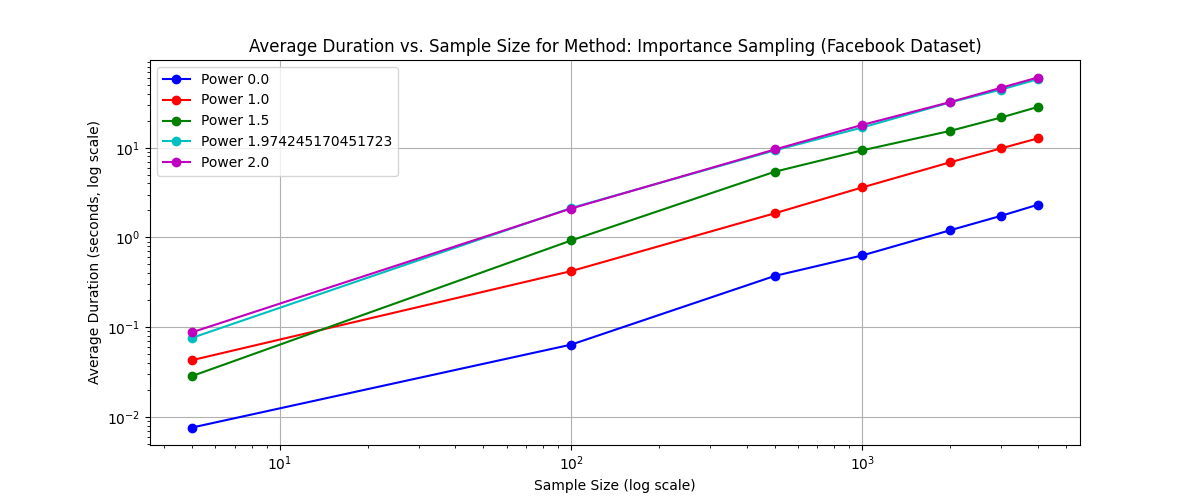
\includegraphics[width=0.8\textwidth]{plots/durations/avg_duration_Importance Sampling.png}
    \caption{Average Duration - Importance Sampling. Runtime increases with sample size and power.}
    \label{fig:avg_duration_importance}
\end{figure}

\begin{figure}[H]
    \centering
    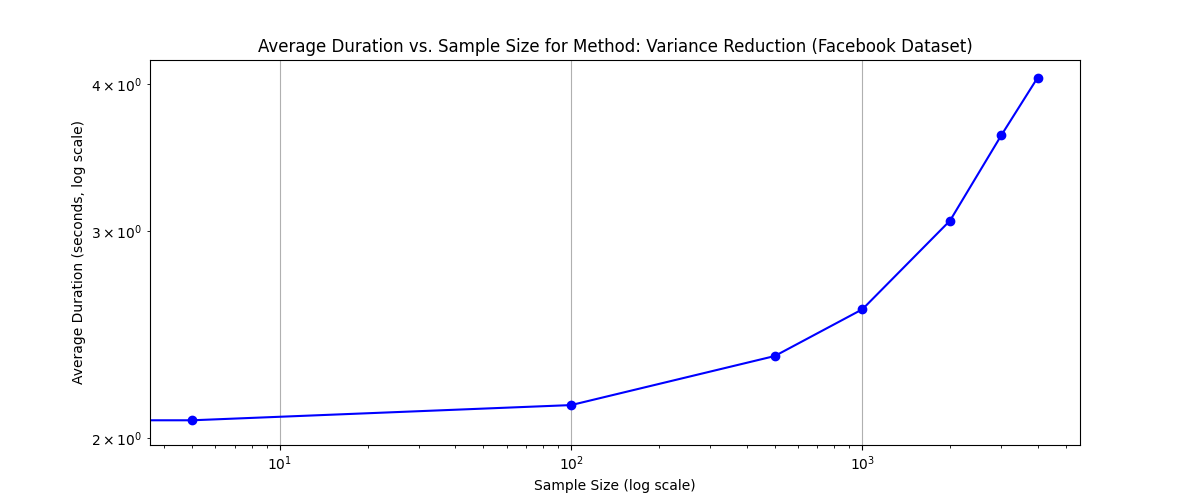
\includegraphics[width=0.8\textwidth]{plots/durations/avg_duration_Variance Reduction.png}
    \caption{Average Duration - Variance Reduction. Runtime increases with sample size.}
    \label{fig:avg_duration_variance}
\end{figure}

\begin{figure}[H]
    \centering
    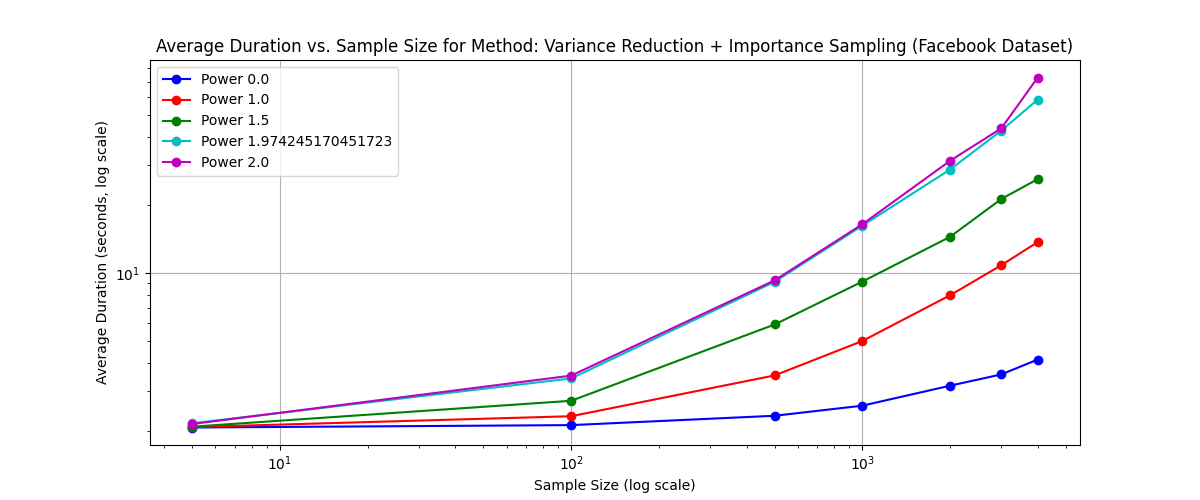
\includegraphics[width=0.8\textwidth]{plots/durations/avg_duration_Variance Reduction + Importance Sampling.png}
    \caption{Average Duration - Variance Reduction + Importance Sampling. Runtime increases with sample size and power.}
    \label{fig:avg_duration_variance_importance}
\end{figure}

\subsubsection{Accuracy and Runtime Comparisons}

This section presents the accuracy and runtime comparisons of different sampling methods across various datasets.
Tables \ref{tab:percent_error_100} and \ref{tab:percent_error_4000} summarize the average percent error for different sampling methods across various datasets with sample sizes of 100 and 4000, respectively.
The most accurate method is highlighted in bold for each dataset.

\begin{table}[ht]
\centering
\caption{Percent Errors for Different Methods on Various Datasets (Sample Size = 100, Power = 2)}
\label{tab:percent_error_100}
\begin{tabular}{|c|c|c|c|c|}
\hline
& \multicolumn{4}{c|}{\textbf{Avg Percent Error}} \\
\hline
\textbf{Dataset} & \textbf{Unif. Sampling} & \textbf{Imp. Sampling} & \textbf{Var. Reduction} & \textbf{Hybrid} \\
\hline
Social Network (FB) & 0.17471 & 0.03741 & 0.18911 & \textbf{0.03267} \\
Collaboration Network & 0.39456 & \textbf{0.04186} & 0.22566 & 0.04470 \\
Wikipedia Article Network & 0.36941 & 0.25732 & 0.85303 & \textbf{0.18180} \\
Barab\'asi--Albert & 0.17220 & 0.01243 & 0.01377 & \textbf{0.00791} \\
\hline
\end{tabular}
\end{table}

\begin{table}[ht]
\centering
\caption{Percent Errors for Different Methods on Various Datasets (Sample Size = 4000, Power = 2)}
\label{tab:percent_error_4000}
\begin{tabular}{|c|c|c|c|c|}
\hline
& \multicolumn{4}{c|}{\textbf{Avg Percent Error}} \\
\hline
\textbf{Dataset} & \textbf{Unif. Sampling} & \textbf{Imp. Sampling} & \textbf{Var. Reduction} & \textbf{Hybrid} \\
\hline
Social Network (FB) & 0.02551 & 0.00608 & 0.05014 & \textbf{0.00482} \\
Collaboration Network & 0.03359 & \textbf{0.00932} & 0.02316 & 0.00944 \\
Wikipedia Article Network & 0.06177 & 0.04821 & 0.14815 & \textbf{0.03789} \\
Barab\'asi--Albert & 0.03299 & 0.00163 & 0.00280 & \textbf{0.00132} \\
\hline
\end{tabular}
\end{table}

Figures \ref{fig:fb_runtime}--\ref{fig:ba_sample_size} provide visual comparisons of percent error versus runtime and percent error versus sample size for multiple datasets.

\newpage

\textbf{Percent Error vs. Runtime}

\begin{figure}[H]
\centering
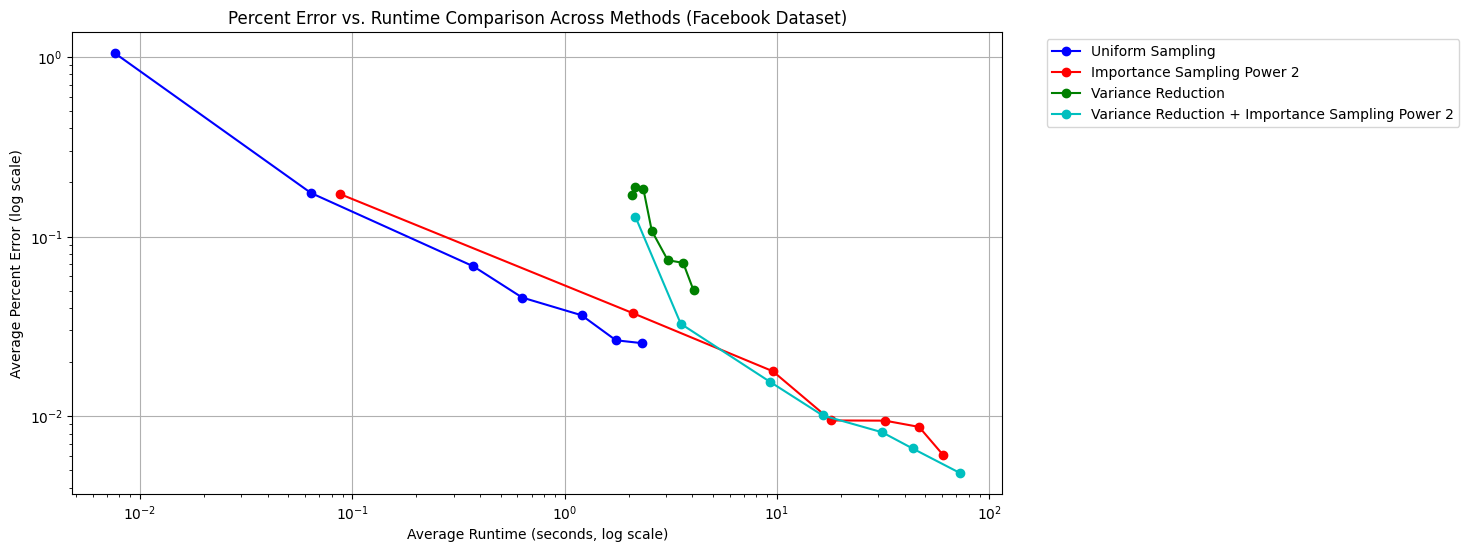
\includegraphics[width=0.9\linewidth]{plots/comparisons/fb/limited_method_percent_error_vs_runtime_comparison.png}
\caption{Percent Error vs. Runtime for Facebook Dataset. Uniform sampling, importance sampling, and the hybrid method have similar errors by runtime, but importance sampling and the hybrid method achieve the lowest errors overall.}
\label{fig:fb_runtime}
\end{figure}

\begin{figure}[H]
\centering
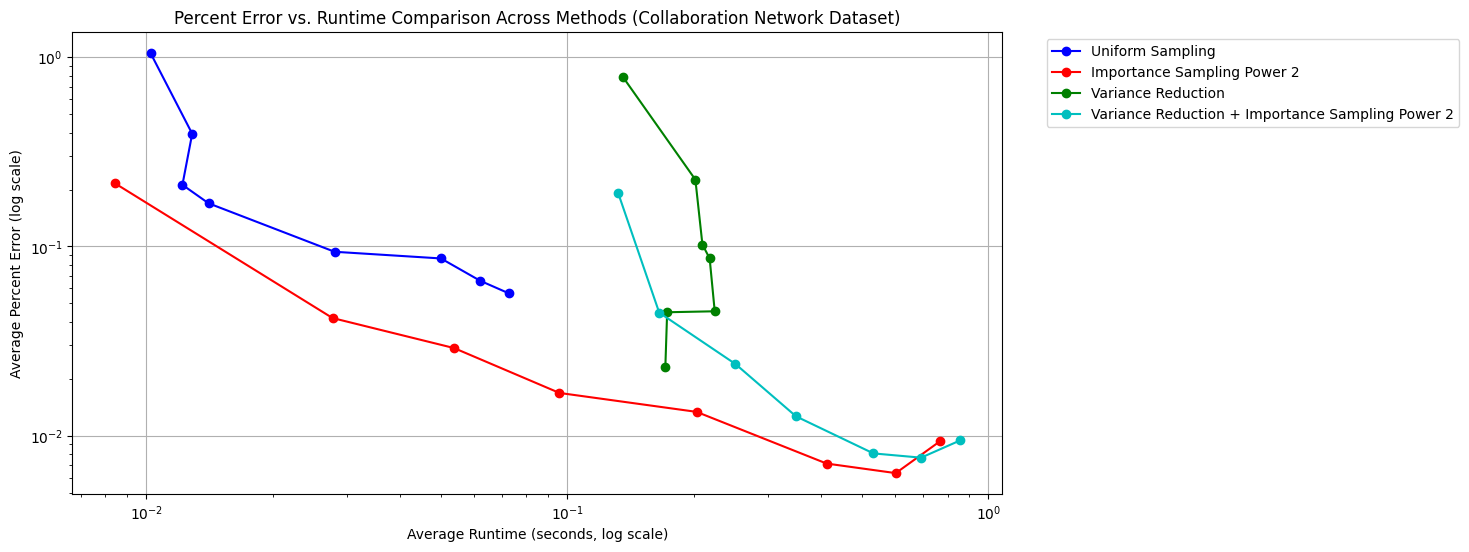
\includegraphics[width=0.9\linewidth]{plots/comparisons/GrQc/limited_method_percent_error_vs_runtime_comparison.png}
\caption{Percent Error vs. Runtime for Collaboration Network Dataset. Importance sampling outperforms other methods.}
\label{fig:grqc_runtime}
\end{figure}

\begin{figure}[H]
\centering
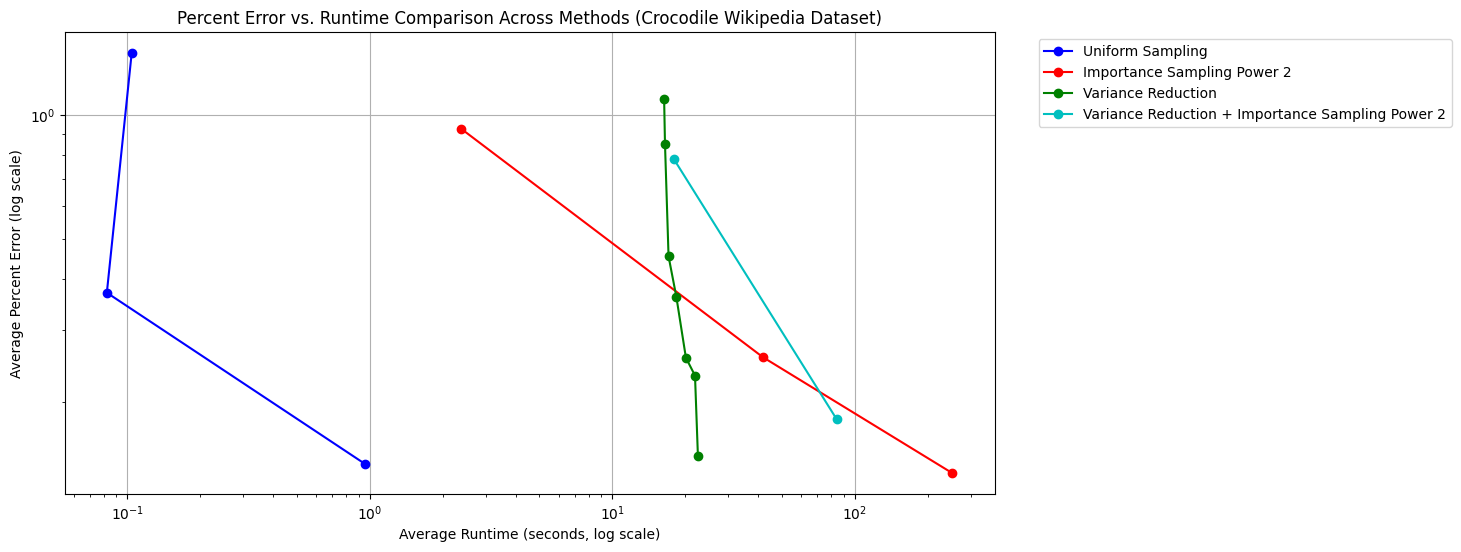
\includegraphics[width=0.9\linewidth]{plots/comparisons/croc/limited_method_percent_error_vs_runtime_comparison.png}
\caption{Percent Error vs. Runtime for Crocodile Wikipedia Dataset. Uniform sampling has a far shorter runtime than the other methods with comparable accuracy for large samples.}
\label{fig:croc_runtime}
\end{figure}

\begin{figure}[H]
\centering
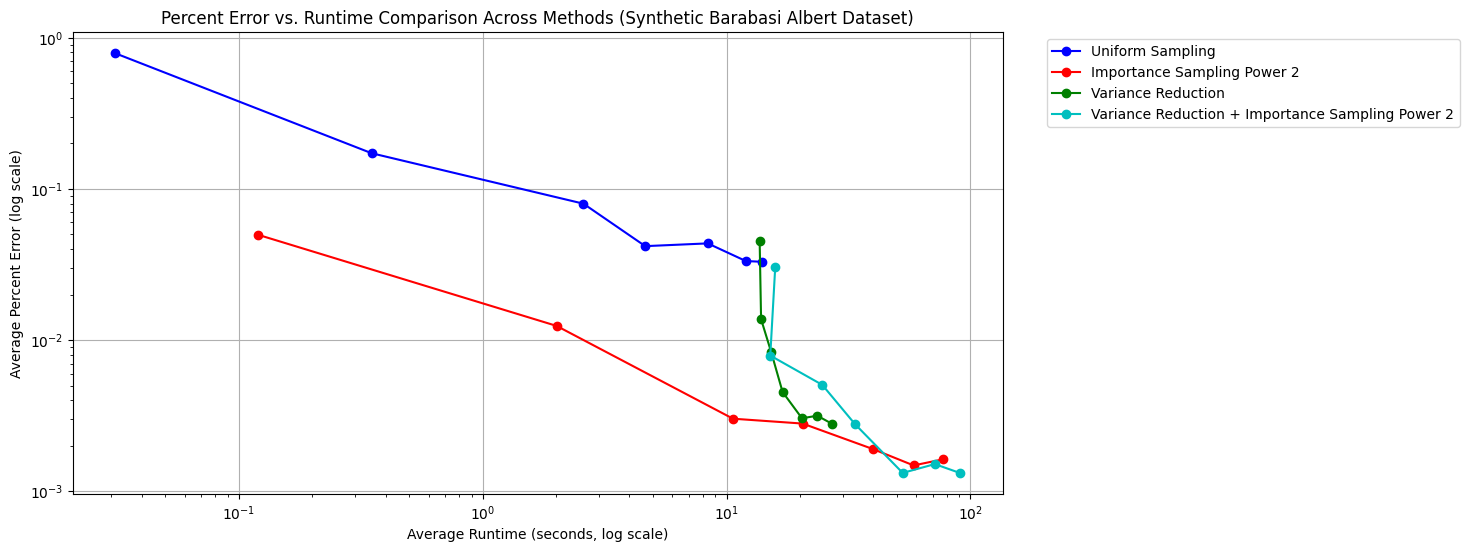
\includegraphics[width=0.9\linewidth]{plots/comparisons/ba/limited_method_percent_error_vs_runtime_comparison.png}
\caption{Percent Error vs. Runtime for Synthetic Barabási–Albert Dataset. The hybrid approach yields the lowest overall error, but for shorter runtimes, importance sampling performs best.}
\label{fig:ba_runtime}
\end{figure}

\textbf{Percent Error vs. Sample Size}

\begin{figure}[H]
\centering
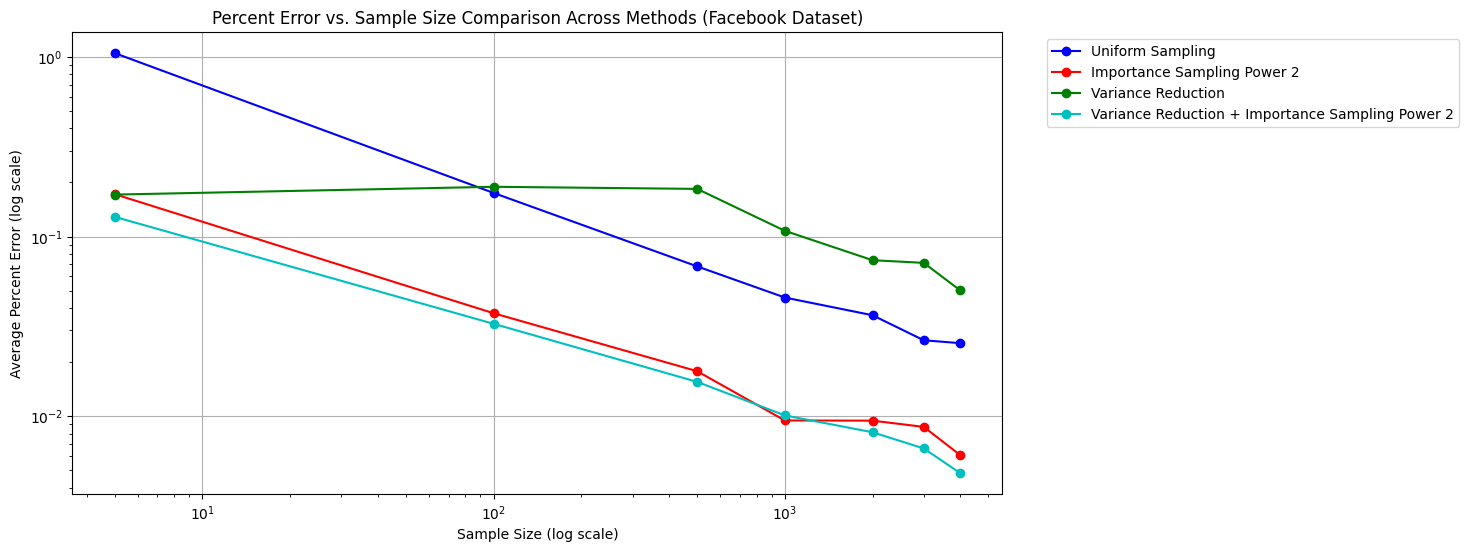
\includegraphics[width=0.9\linewidth]{plots/comparisons/fb/limited_method_percent_error_vs_sample_size_comparison.png}
\caption{Percent Error vs. Sample Size for Facebook Dataset. Importance sampling and the hybrid approach perform best, with the hybrid method performing slightly better.}
\label{fig:fb_sample_size}
\end{figure}

\begin{figure}[H]
\centering
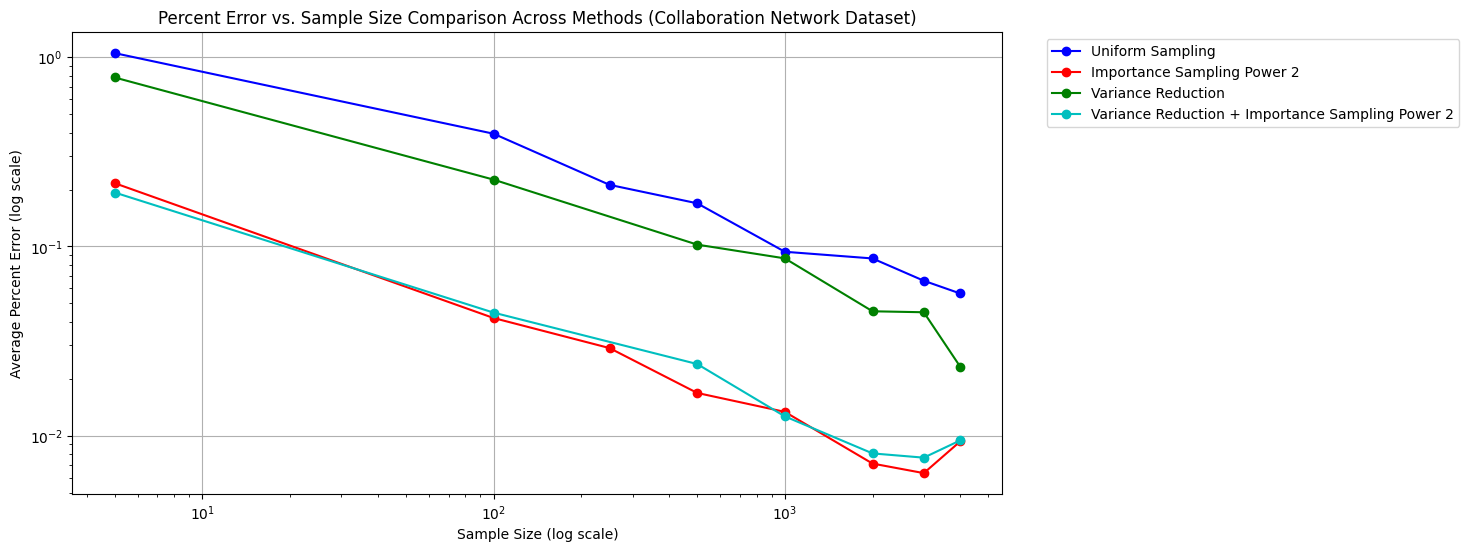
\includegraphics[width=0.9\linewidth]{plots/comparisons/GrQc/limited_method_percent_error_vs_sample_size_comparison.png}
\caption{Percent Error vs. Sample Size for Collaboration Network Datase. Importance sampling and the hybrid approach perform best.}
\label{fig:grqc_sample_size}
\end{figure}

\begin{figure}[H]
\centering
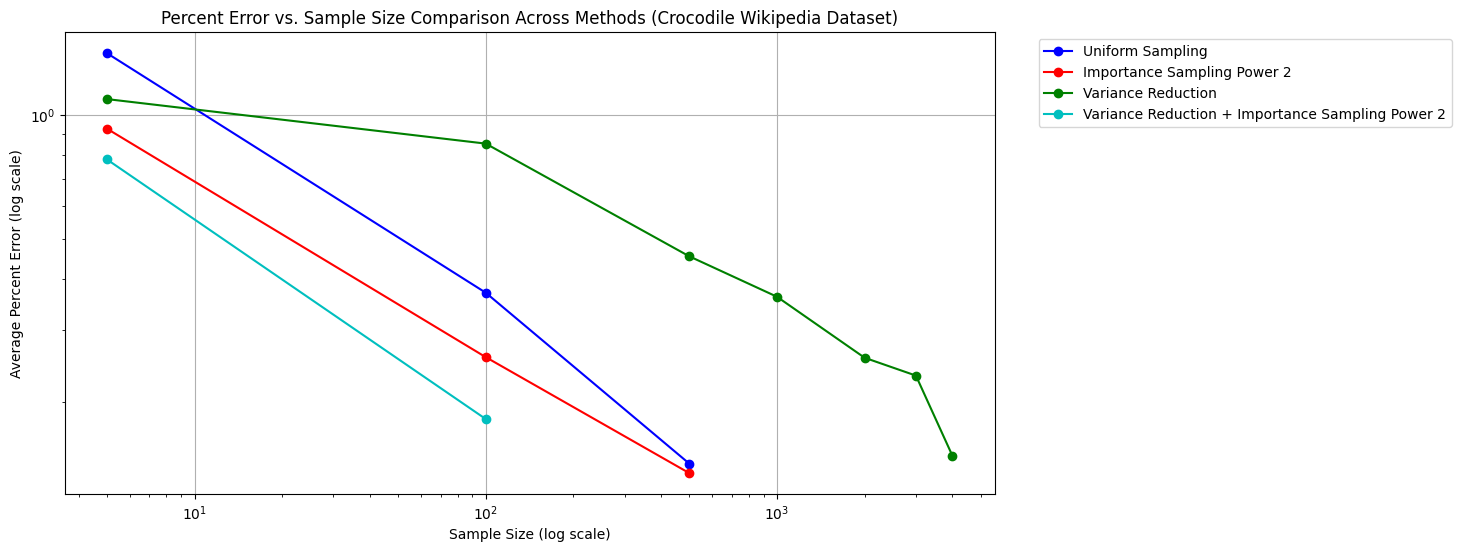
\includegraphics[width=0.9\linewidth]{plots/comparisons/croc/limited_method_percent_error_vs_sample_size_comparison.png}
\caption{Percent Error vs. Sample Size for Crocodile Wikipedia Dataset. The hybrid method performs best.}
\label{fig:croc_sample_size}
\end{figure}

\begin{figure}[H]
\centering
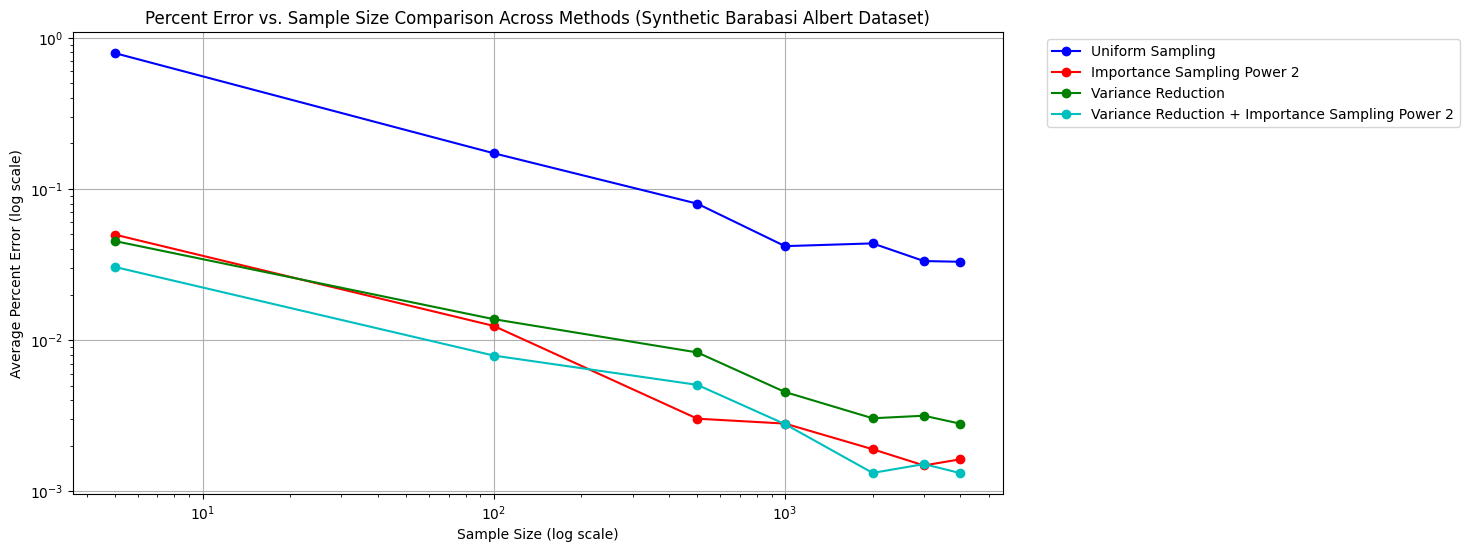
\includegraphics[width=0.9\linewidth]{plots/comparisons/ba/limited_method_percent_error_vs_sample_size_comparison.png}
\caption{Percent Error vs. Sample Size for Synthetic Barabási–Albert Dataset. Importance sampling, variance reduction, and the hybrid method perform best, with importance sampling and the hybrid method performing best.}
\label{fig:ba_sample_size}
\end{figure}

\subsection{4-Clique Counting}

In this section, we present the results of our experiments on 4-clique counting.
We compare importance sampling and variance reduction, and illustrate how the power in importance sampling impacts percent error, sample size, and runtime in 4-clique counting.
All shown results are from the Collaboration Network dataset.

\begin{figure}[H]
    \centering
    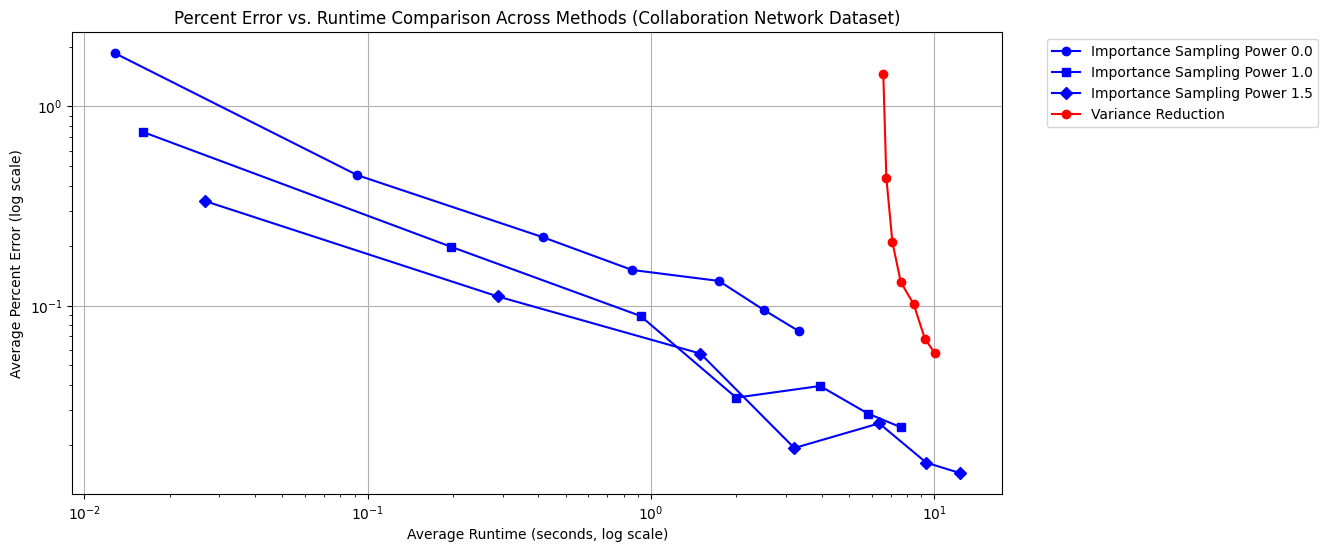
\includegraphics[width=0.8\textwidth]{plots/4-clique/comparison/percent_error_vs_runtime_comparison.png}
    \caption{Comparison of percent error versus runtime for different methods in 4-clique counting. Importance sampling with higher powers outperforms variance reduction.}
    \label{fig:4_clique_percent_error_runtime_comparison}
\end{figure}

\begin{figure}[H]
    \centering
    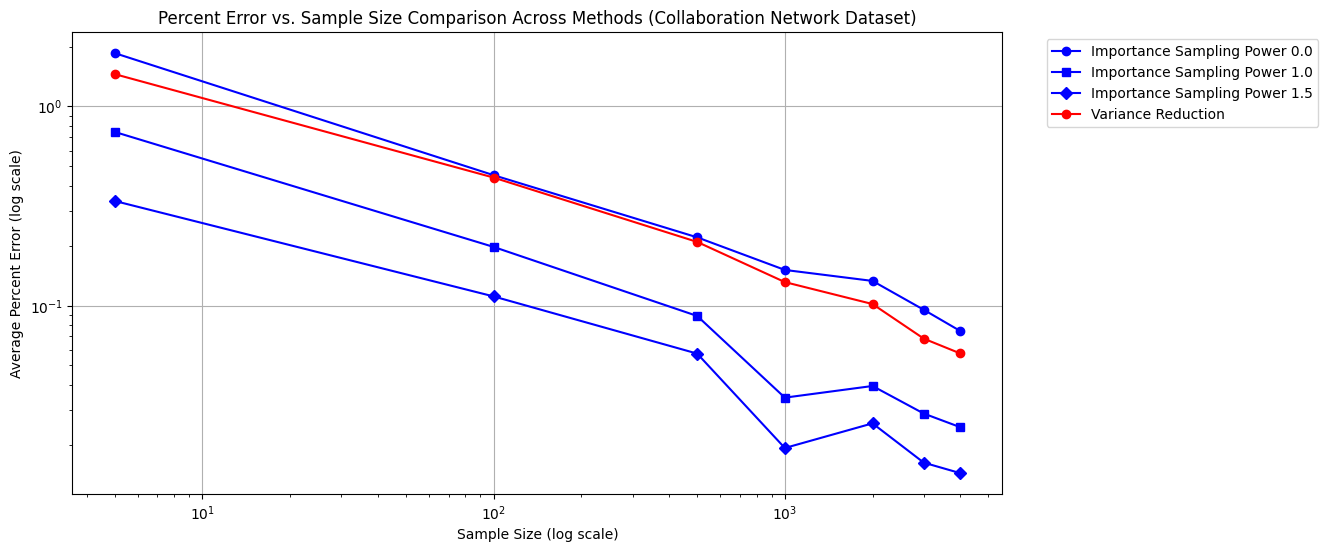
\includegraphics[width=0.8\textwidth]{plots/4-clique/comparison/percent_error_vs_sample_size_comparison.png}
    \caption{Comparison of percent error versus sample size for different 4-clique counting methods. Importance sampling with higher powers outperforms variance reduction.}
    \label{fig:4_clique_percent_error_sample_size_comparison}
\end{figure}

\begin{figure}[H]
    \centering
    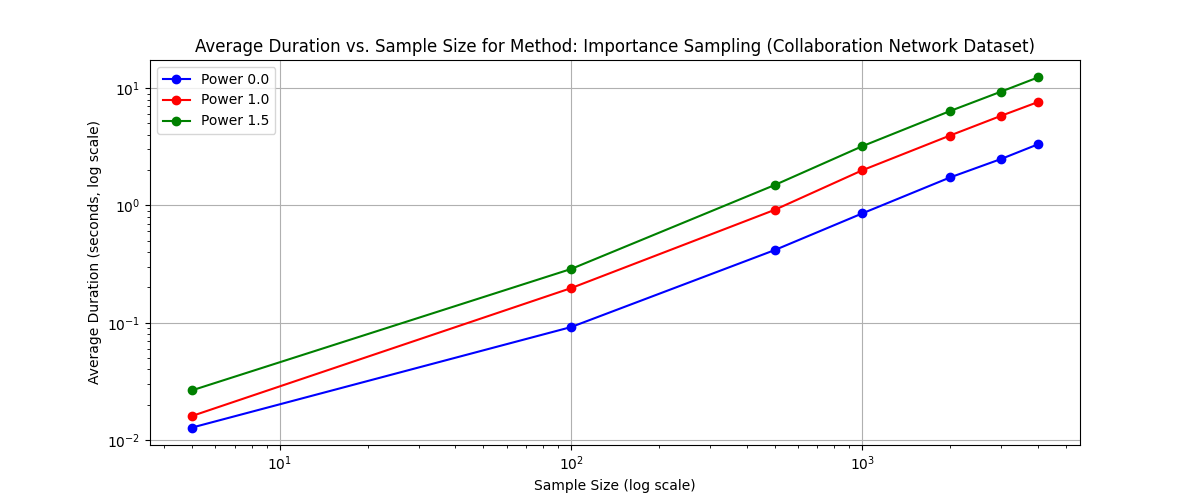
\includegraphics[width=0.8\textwidth]{plots/4-clique/importance-sampling/avg_duration_Importance Sampling.png}
    \caption{Average duration of the importance sampling method across powers for 4-clique counting. Runtime increases with sample size and power.}
    \label{fig:4_clique_avg_duration_importance_sampling}
\end{figure}

\begin{figure}[H]
    \centering
    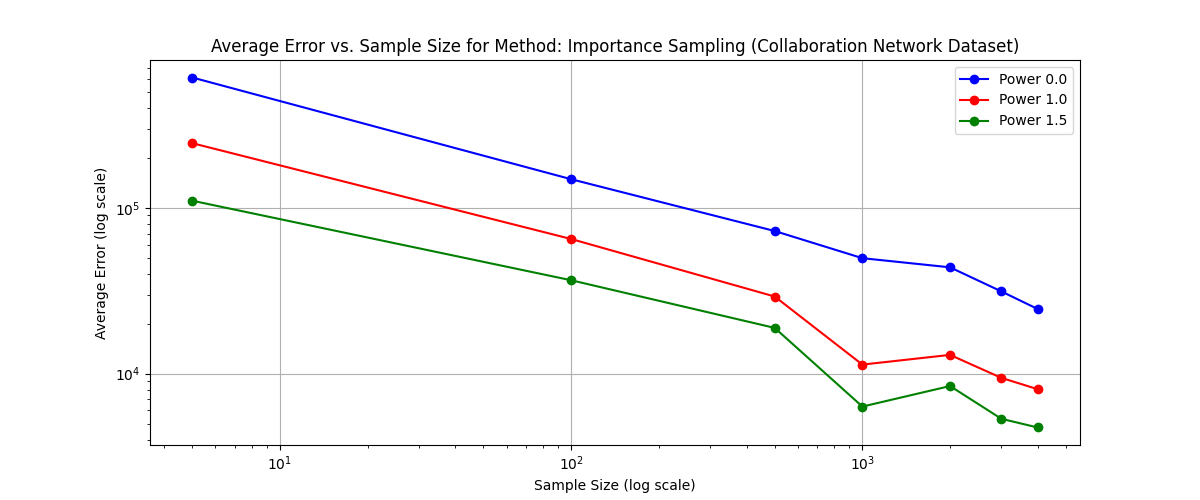
\includegraphics[width=0.8\textwidth]{plots/4-clique/importance-sampling/avg_error_Importance Sampling.png}
    \caption{Average error of the importance sampling method across powers for 4-clique counting. Average error decreases as sample size increases. The power of 1.5 performs best.}
    \label{fig:4_clique_avg_error_importance_sampling}
\end{figure}

\subsection{Simulated Method Tests}

To assess the performance of importance sampling and variance reduction, we tested these algorithms under two different triangle-degree relationships: uniform noise and multiplicative noise.
In this section, we present the results of these tests, focusing on the relationship between sample size and average error for both types of noise across various scales.

\subsubsection{Uniform Noise Relationship}

In this subsection, we examine the performance of the algorithms with uniform noise.
The degree distribution was derived from the Collaboration Network dataset, and the triangle counts were generated using the formula:

\[
\text{triangle counts} = \text{np.power(degrees, slope)} \times \text{np.exp(intercept)} + \text{noise},
\]

where \text{noise} is normally distributed with mean zero and standard deviation defined by three scales: 10, 100, and 500. The following figures display the relationship between sample size and average error for each of these noise scales.

\begin{figure}[H]
    \centering
    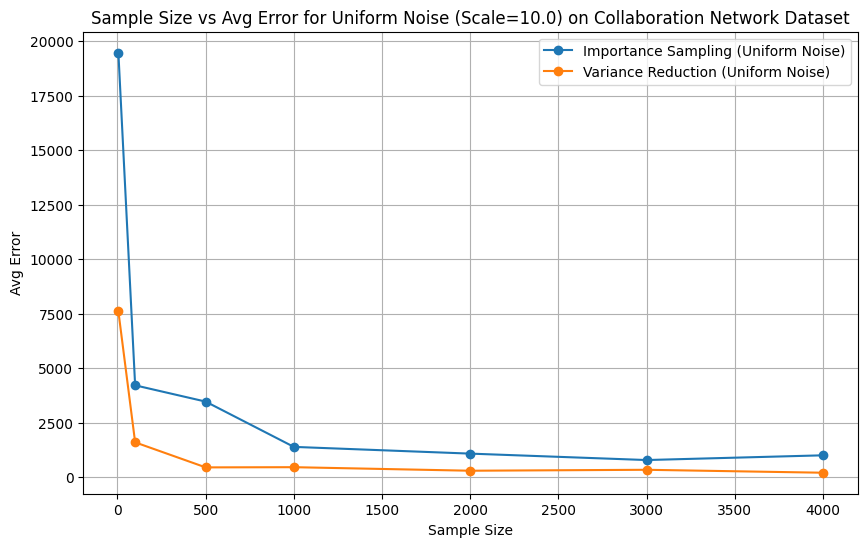
\includegraphics[width=0.7\textwidth]{plots/simulated/percent_error_vs_sample_size_comparison_uniform_10.0.png}
    \caption{Sample size vs. average error with uniform noise (scale = 10). Variance reduction outperforms importance sampling.}
    \label{fig:uniform_noise_10}
\end{figure}

\begin{figure}[H]
    \centering
    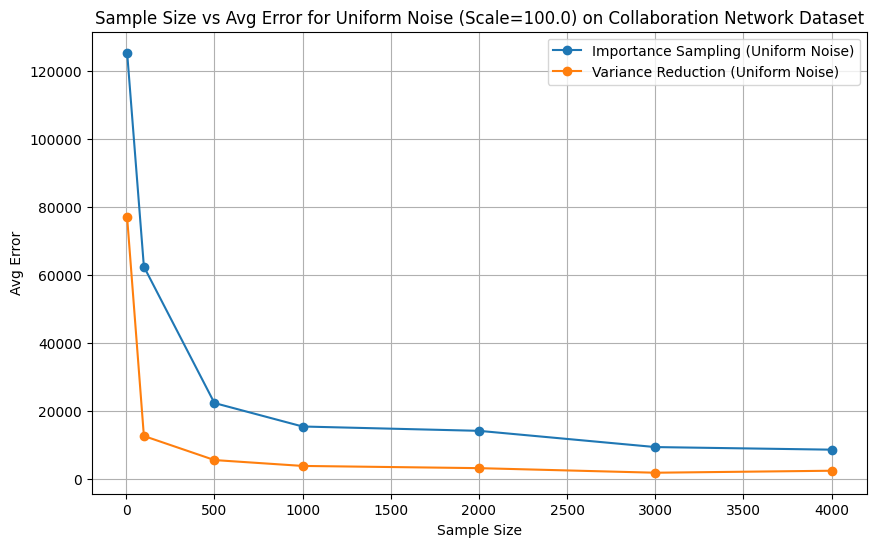
\includegraphics[width=0.7\textwidth]{plots/simulated/percent_error_vs_sample_size_comparison_uniform_100.0.png}
    \caption{Sample size vs. average error with uniform noise (scale = 100). Variance reduction outperforms importance sampling.}
    \label{fig:uniform_noise_100}
\end{figure}

\begin{figure}[H]
    \centering
    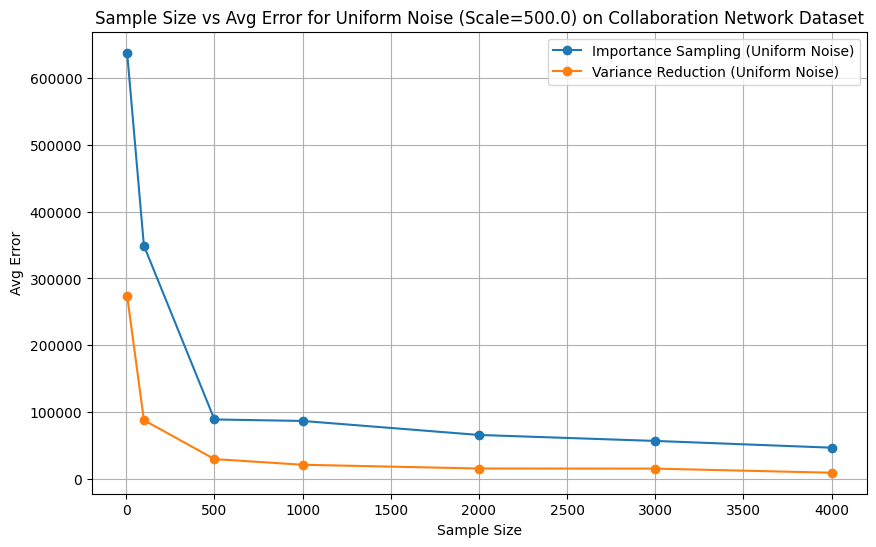
\includegraphics[width=0.7\textwidth]{plots/simulated/percent_error_vs_sample_size_comparison_uniform_500.0.png}
    \caption{Sample size vs. average error with uniform noise (scale = 500). Variance reduction outperforms importance sampling.}
    \label{fig:uniform_noise_500}
\end{figure}

\subsubsection{Multiplicative Noise Relationship}

Next, we consider the performance of the algorithms with multiplicative noise. The triangle counts were generated using the following formula:

\[
\text{triangle counts} = \text{np.power(degrees, slope)} \times \text{np.exp(intercept)} \times (1 + \text{noise}),
\]

where \text{noise} is again normally distributed and grows with the degree, and the noise scale was tested at three values: 0.01, 0.1, and 0.5. Below are the figures for sample size vs. average error for each noise scale in the multiplicative noise case.

\begin{figure}[H]
    \centering
    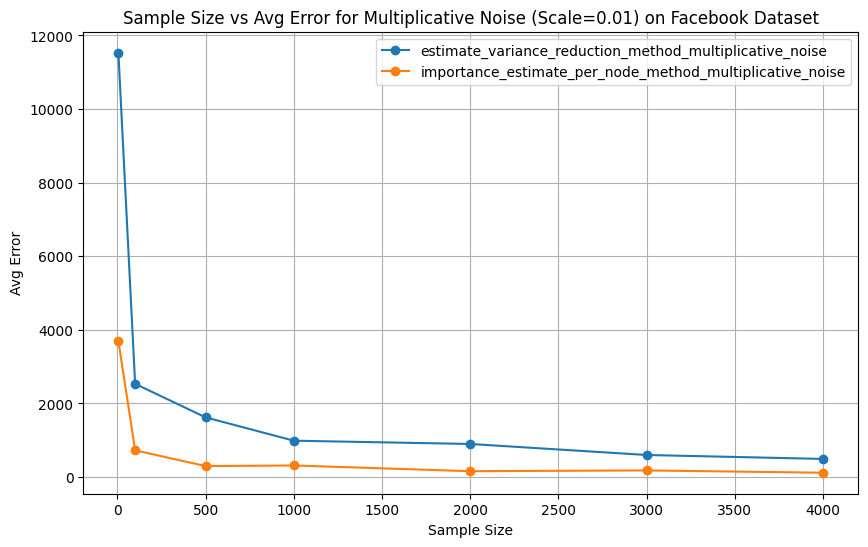
\includegraphics[width=0.7\textwidth]{plots/simulated/percent_error_vs_sample_size_comparison_multiplicative_0.01.png}
    \caption{Sample size vs. average error with multiplicative noise (scale = 0.01). Importance sampling outperforms variance reduction.}
    \label{fig:multiplicative_noise_001}
\end{figure}

\begin{figure}[H]
    \centering
    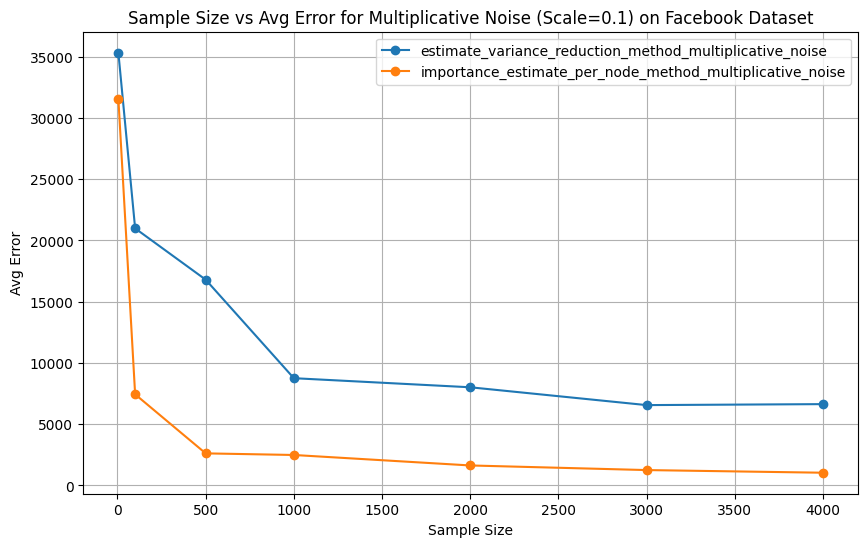
\includegraphics[width=0.7\textwidth]{plots/simulated/percent_error_vs_sample_size_comparison_multiplicative_0.1.png}
    \caption{Sample size vs. average error with multiplicative noise (scale = 0.1). Importance sampling outperforms variance reduction.}
    \label{fig:multiplicative_noise_01}
\end{figure}

\begin{figure}[H]
    \centering
    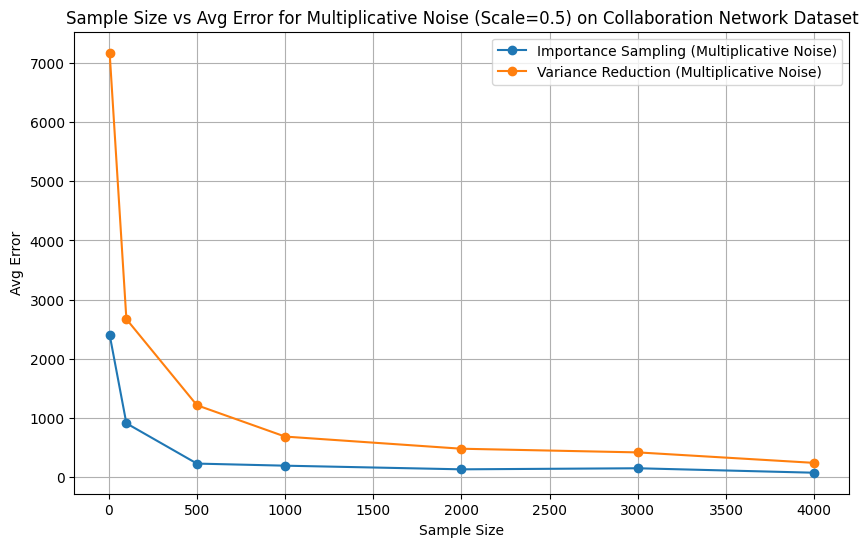
\includegraphics[width=0.7\textwidth]{plots/simulated/percent_error_vs_sample_size_comparison_multiplicative_0.5.png}
    \caption{Sample size vs. average error with multiplicative noise (scale = 0.5). Importance sampling outperforms variance reduction.}
    \label{fig:multiplicative_noise_05}
\end{figure}

\newpage

\section{Discussion}

TODO: PUT THIS IN THE CORRECT LOCATION:

As illustrated in figures \ref{fig:avg_duration_importance} and \ref{fig:avg_duration_variance_importance}, larger powers lead to higher runtimes.
In figures \ref{fig:percent_error_importance} and \ref{fig:percent_error_variance_importance}, we see that powers closest to the optimal value $\alpha$, as described in section \ref{sec:importance-sampling-background} have lowest percent error.
In the case of the Social Network (Facebook) dataset, this value is $\alpha \approx 1.97$.

However, we also see in figures \ref{fig:percent_error_importance} and \ref{fig:percent_error_variance_importance} that after a certain point, the decrease in percent error by power is very slight.
For both importance sampling and the hybrid method, powers of 1.5, 2, and $~ 1.97$ all perform about the same.
Thus, while a higher power may yield the lowest error, in practical applications, it may make more sense to take a slightly lower power to decrease runtime.

TODO INTRODUCE THIS AND CONNECT IT TO SIMULATED TESTS

\begin{figure}[H]
    \centering

    \begin{subfigure}[b]{0.49\textwidth}
        \centering
        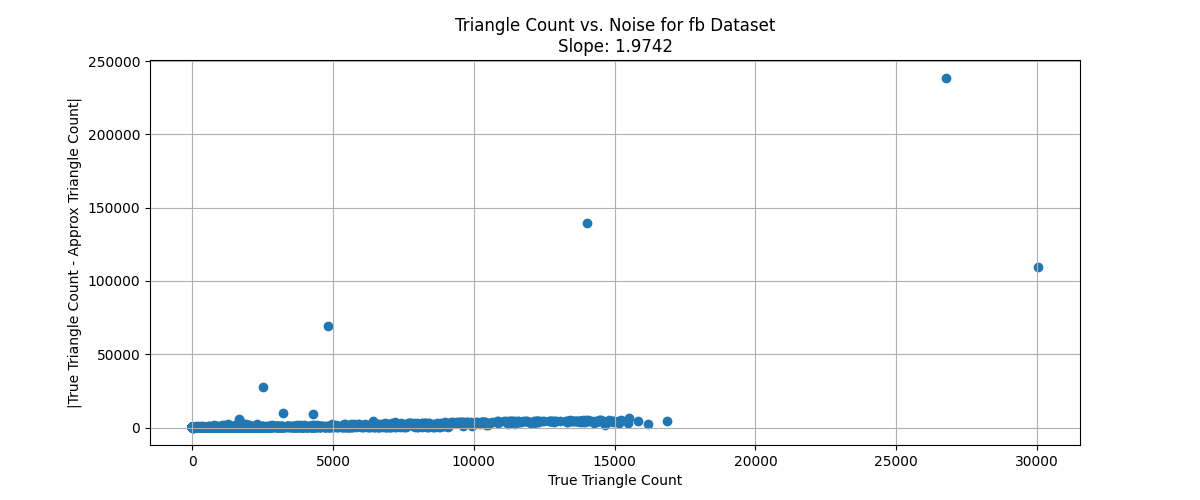
\includegraphics[width=\textwidth]{plots/triangle-counts-vs-noise/fb_triangle_count_vs_noise.png}
        \caption{Facebook}
        \label{fig:tri_vs_noise_fb}
    \end{subfigure}
    \hfill
    \begin{subfigure}[b]{0.49\textwidth}
        \centering
        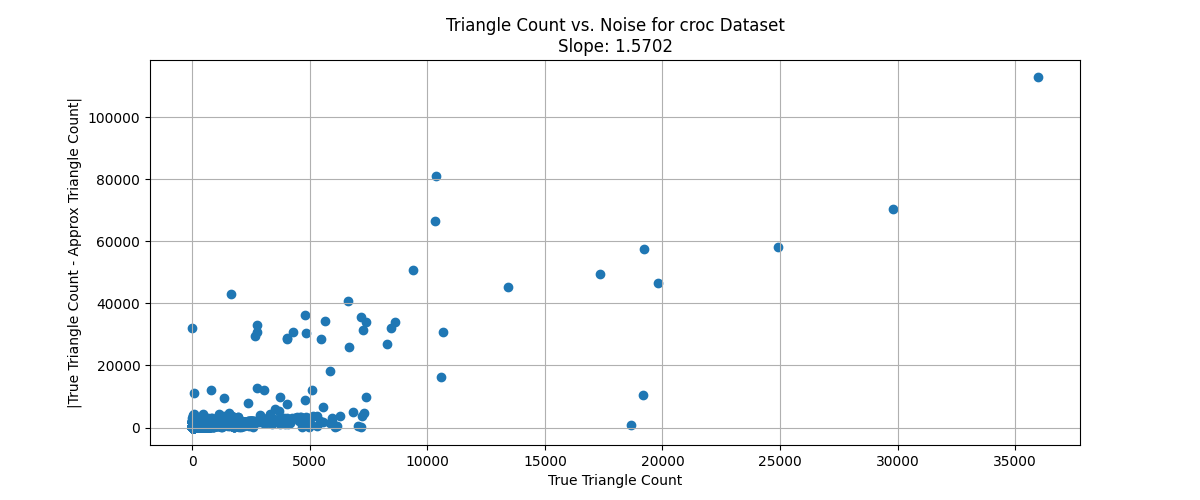
\includegraphics[width=\textwidth]{plots/triangle-counts-vs-noise/croc_triangle_count_vs_noise.png}
        \caption{Wikipedia}
        \label{fig:tri_vs_noise_croc}
    \end{subfigure}
    \hfill
    \begin{subfigure}[b]{0.49\textwidth}
        \centering
        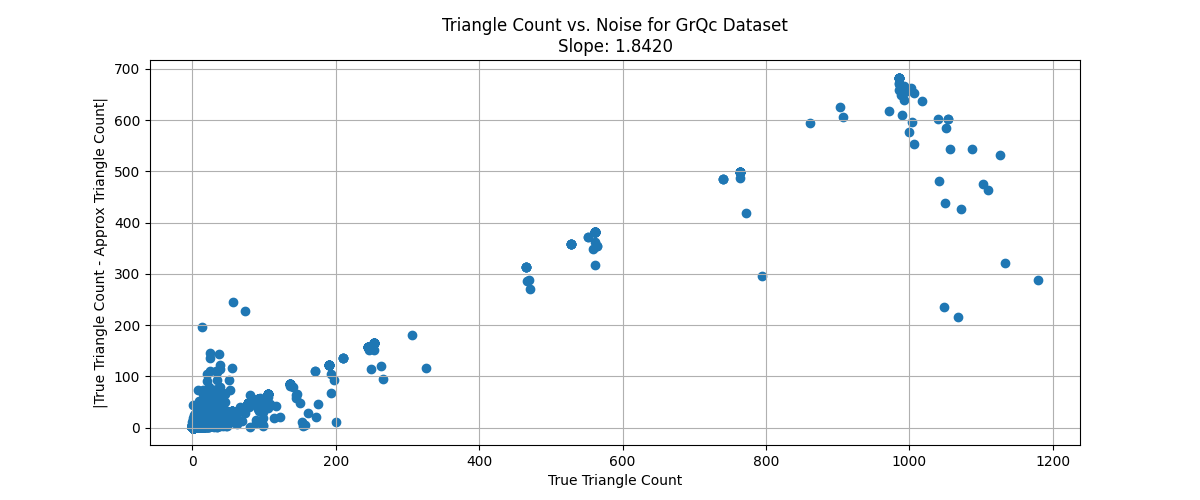
\includegraphics[width=\textwidth]{plots/triangle-counts-vs-noise/GrQc_triangle_count_vs_noise.png}
        \caption{Collaboration}
        \label{fig:tri_vs_noise_GrQc}
    \end{subfigure}
    \hfill
    \begin{subfigure}[b]{0.49\textwidth}
        \centering
        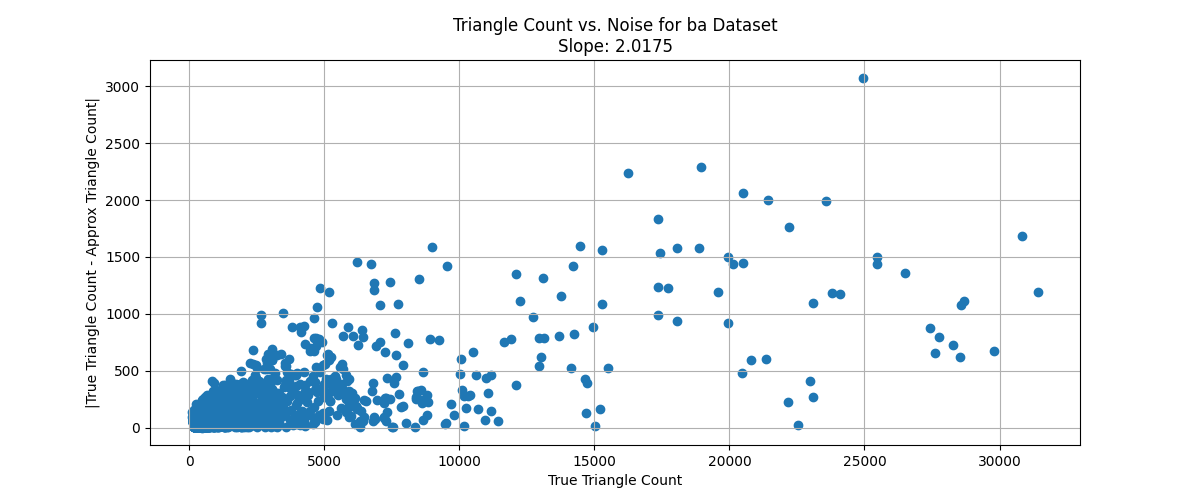
\includegraphics[width=\textwidth]{plots/triangle-counts-vs-noise/ba_triangle_count_vs_noise.png}
        \caption{Barabási–Albert}
        \label{fig:tri_vs_noise_ba}
    \end{subfigure}

    \caption{Triangle counts vs. noise across all datasets. Nodes with higher triangle counts often have higher noise.}
    \label{fig:tri_vs_noise}
\end{figure}

\subsection{Theoretical Analysis of Variances}

Understanding the variance of the algorithms tested is crucial for evaluating their reliability.
Thus, in this section, we derive expressions for the variance of the estimated triangle count across methods.

\subsubsection{Uniform Sampling}

The global triangle count $\Delta$ can be estimated as $\tilde{\Delta}$ using the following formula:

\[
\tilde{\Delta} = \frac{n}{3s} \sum_{i = 1}^{s} \Delta_i,
\]

where $n$ is the number of nodes in our graph $G$, $s$ is our sample size, and $\sum_{i = 1}^{s} \Delta_i$ is the sum of all sampled triangle counts. 
Using this, we can find the variance of $\tilde{\Delta}$ in terms of $n$, $s$, and $\mathrm{Var}(\Delta_i)$.

\[
\begin{aligned}
\mathrm{Var}(\tilde{\Delta}) &= \mathrm{Var} \left( \frac{n}{3s} \sum_{i=1}^{s} \Delta_i \right) \\
&= \frac{n^2}{9s^2} \mathrm{Var} \left( \sum_{i=1}^{s} \Delta_i \right) \\
&= \frac{n^2}{9s^2} \sum_{i=1}^{s} \mathrm{Var}(\Delta_i)
\end{aligned}
\]

Next, we find $\mathrm{Var}(\Delta_i)$.

\[
\mathrm{Var}(\Delta_i) = \mathbb{E}[(\Delta_i - \mathbb{E}[\Delta_i])^2]
\]

\[
\mathbb{E}[\Delta_i] = 3(\frac{1}{n} \Delta_1 + \frac{1}{n} \Delta_2 + \ldots + \frac{1}{n} \Delta_n) = \frac{3\Delta}{n}
\]

\[
\begin{aligned}
\mathbb{E}[(\Delta_i - \mathbb{E}[\Delta_i])^2] &= \mathbb{E}[(\Delta_i - \frac{3\Delta}{n})^2] \\
&= \sum_{i = 1}^{n} \frac{1}{n} (\Delta_i - \frac{3\Delta}{n})^2 \\
&= \sum_{i = 1}^{n} \frac{1}{n} (\Delta_i^2 - 6 \Delta_i \frac{\Delta}{n} + \frac{9\Delta^2}{n^2}) \\
&= \frac{1}{n} \sum_{i = 1}^{n} \Delta_i^2 - \frac{6}{n} \sum_{i = 1}^{n} \Delta_i \frac{\Delta}{n} + \frac{1}{n} \sum_{i = 1}^{n} \frac{9\Delta^2}{n^2} \\
&= \frac{1}{n} \sum_{i = 1}^{n} \Delta_i^2 - \frac{6}{n} \sum_{i = 1}^{n} \Delta_i \frac{\Delta}{n} + \frac{9\Delta^2}{n^2} \\
&= \frac{1}{n} \sum_{i = 1}^{n} \Delta_i^2 - \frac{18\Delta^2}{n^2} + \frac{9\Delta^2}{n^2} \\
&= \frac{1}{n} \sum_{i = 1}^{n} \Delta_i^2 - \frac{9\Delta^2}{n^2}
\end{aligned}
\]

Now, we can plug our value of $\mathrm{Var}(\Delta_i)$ into $\mathrm{Var}(\tilde{\Delta}) = \frac{n^2}{9s^2} \sum_{i=1}^{s} \mathrm{Var}(\Delta_i)$.

\[
\begin{aligned}
\mathrm{Var}(\tilde{\Delta}) &= \frac{n^2}{9s^2} \sum_{i=1}^{s} [\frac{1}{n} \sum_{i = 1}^{n} \Delta_i^2 - \frac{9\Delta^2}{n^2}] \\
&= \frac{n^2}{9s^2} s [\frac{1}{n} \sum_{i = 1}^{n} \Delta_i^2 - \frac{9\Delta^2}{n^2}] \\
&= \frac{n^2}{9s} [\frac{1}{n} \sum_{i = 1}^{n} \Delta_i^2 - \frac{9\Delta^2}{n^2}] \\
&= \frac{n}{s} [\frac{1}{9}\sum_{i = 1}^{n} \Delta_i^2 - \frac{\Delta^2}{n}] \\
&= \frac{n}{9s} \sum_{i = 1}^{n} \Delta_i^2 - \frac{\Delta^2}{s} \\
\end{aligned}
\]

\subsubsubsection{Importance Sampling}

The global triangle count $\Delta$ can be estimated as $\tilde{\Delta}$ using the following formula:

\[
\tilde{\Delta} = \frac{1}{3s} \sum_{j = 1}^{s} \frac{\Delta_{ij}}{p_{ij}},
\]

where $p_i = \frac{m_i}{\sum_{j = 1}^{n}m_{ij}}$ with $m_j = \Delta_j + n_j$ where $n_i \in [-\sigma \Delta_i, \sigma \Delta_i]$ and $\sigma < 1$.

\[
\begin{aligned}
\mathrm{Var}(\tilde{\Delta}) &= \mathrm{Var} \left( \frac{1}{3s} \sum_{j = 1}^{s} \frac{\Delta_{ij}}{p_{ij}} \right) \\
&= \frac{1}{9s^2} \mathrm{Var} \left( \sum_{j = 1}^{s} \frac{\Delta_{ij}}{p_{ij}} \right) \\
&= \frac{1}{9s^2} \sum_{j = 1}^{s} \mathrm{Var} \left( \frac{\Delta_{ij}}{p_{ij}} \right) \\
&= \frac{1}{9s^2} \sum_{j = 1}^{s} [\mathbb{E}[(\frac{\Delta_{ij}}{p_{ij}})^2] - (\mathbb{E}[\frac{\Delta_{ij}}{p_{ij}}])^2] \\
&= \frac{1}{9s^2} \sum_{j = 1}^{s} [\mathbb{E}[(\frac{\Delta_{ij}}{p_{ij}})^2] - (\sum_{n}^{j=1}(p_j \frac{\Delta_j}{p_j}))^2] \\
&= \frac{1}{9s^2} \sum_{j = 1}^{s} [\mathbb{E}[(\frac{\Delta_{ij}}{p_{ij}})^2] - (\sum_{n}^{j=1}\Delta_j)^2] \\
&= \frac{1}{9s^2} \sum_{j = 1}^{s} [\mathbb{E}[(\frac{\Delta_{ij}}{p_{ij}})^2] - \Delta^2] \\
&= \frac{1}{9s^2} \sum_{j = 1}^{s} [\sum_{j = 1}^{n}(p_j \frac{\Delta_j^2}{p_j^2}) - \Delta^2] \\
&= \frac{1}{9s^2} \sum_{j = 1}^{s} [\sum_{j = 1}^{n}(\frac{\Delta_j^2}{p_j}) - \Delta^2] \\
&= \frac{1}{9s^2} \sum_{j = 1}^{s} [\sum_{j = 1}^{n}\frac{\Delta_j^2}{m_j} \sum_{i = 1}^{n}m_i - \Delta^2] \\
&= \frac{1}{9s^2} \sum_{j = 1}^{s} [\sum_{i = 1}^{n}m_i \sum_{j = 1}^{n}\frac{\Delta_j^2}{m_j} - \Delta^2] \\
\end{aligned}
\]

We can set an upper bound on $\sum_{i = 1}^{n}m_i$ as follows:

\[
\begin{aligned}
\sum_{i = 1}^{n}m_i &\leq \sum_{i = 1}^{n}(\Delta_i + \sigma \Delta_i) \\
&\leq (1 + \sigma) \Delta \\
\end{aligned}
\]

We can similarly set an upper bound on $\sum_{j = 1}^{n}\frac{\Delta_j^2}{m_j}$ as follows:

\[
\begin{aligned}
\sum_{j = 1}^{n}\frac{\Delta_j^2}{m_j} &\leq \sum_{j = 1}^{n}\frac{\Delta_j^2}{(1 - \sigma) \Delta_j} \\
&= \sum_{j = 1}^{n}\frac{\Delta_j}{1 - \sigma} \\
&= \frac{1}{1 - \sigma} \sum_{j = 1}^{n}\Delta_j \\
&= \frac{1}{1 - \sigma} \Delta \\
\end{aligned}
\]

Combining these two bounds we can return to our variance expression:

\[
\begin{aligned}
\mathrm{Var}(\tilde{\Delta}) &= \frac{1}{9s^2} \sum_{j = 1}^{s} [\sum_{i = 1}^{n}m_i \sum_{j = 1}^{n}\frac{\Delta_j^2}{m_j} - \Delta^2] \\
&\leq \frac{1}{9s^2} \sum_{j = 1}^{s} [\frac{1 + \sigma}{1 - \sigma} \Delta^2 - \Delta^2] \\
&= \frac{1}{9s^2} \sum_{j = 1}^{s} [(\frac{1 + \sigma}{1 - \sigma} - 1) \Delta^2] \\
&= \frac{1}{9s} (\frac{1 + \sigma}{1 - \sigma} - 1) \Delta^2 \\
\end{aligned}
\]

\subsubsection{Variance Reduction}

Across this section, we will use the fact that $\mathrm{Var}[X+Y] \leq 2(\mathrm{Var}[X] + \mathrm{Var}[Y])$. We derive that as follows:

\[
\begin{aligned}
    \mathrm{Var}[X+Y] &= \mathbb{E}[(X+Y)^2] \\
    &= \mathbb{E}[X^2] + \mathbb{E}[Y^2] + 2\mathbb{E}[XY] \\
    &\leq \mathbb{E}[X^2] + \mathbb{E}[Y^2] + (\mathbb{E}[X^2] + \mathbb{E}[Y^2]) \\
    &= 2(\mathbb{E}[X^2] + \mathbb{E}[Y^2]) \\
    &= 2(\mathrm{Var}[X] + \mathrm{Var}[Y])
\end{aligned}
\]

\subsubsubsection{Variance Reduction with Uniform Noise}

Take the estimator of $\Delta$ to be denoted by $M$ where $M = \sum_{i = 1}^{n} m_i$ and $m_i = \Delta_i + N(0, \sigma^2)$.

\[
\tilde{\Delta} = \sum_{i = 1}^{n} m_i + \frac{n}{s} \sum_{i = 1}^{s} (m_i - \Delta_i)
\]

\[
\begin{aligned}
\mathrm{Var}(\tilde{\Delta}) &= \mathrm{Var}( \sum_{i = 1}^{n} m_i + \frac{n}{s} \sum_{i = 1}^{s} (m_i - \Delta_i)) \\
&\leq 2\sum_{i = 1}^{n} \mathrm{Var}(m_i) + 2\mathrm{Var}(\frac{n}{s} \sum_{i = 1}^{s} (m_i - \Delta_i)) \\
&= 2\sum_{i = 1}^{n} \mathrm{Var}(m_i) + \frac{2n^2}{s^2} \mathrm{Var}(\sum_{i = 1}^{s} (m_i - \Delta_i)) \\
&= 2\sum_{i = 1}^{n} \mathrm{Var}(m_i) + \frac{2n^2}{s^2} \sum_{i = 1}^{s} \mathrm{Var}(m_i - \Delta_i) \\
&= 2n \sigma^2 + \frac{2n^2}{s^2} \sum_{i = 1}^{s} \mathrm{Var}(m_i - \Delta_i) \\
&= 2n \sigma^2 + \frac{2n^2}{s^2} s \sigma^2 \\
&= 2n \sigma^2 + \frac{2n^2}{s} \sigma^2 \\
\end{aligned}
\]

To allow for better comparison with other methods, assume $\sigma^2$ is the average squared error when using the trivial predictor of $m_i = 0$.
In this case, $\sigma^2 = \frac{\sum_{i = 1}^{n}\Delta_i^2}{n}$.

Plugging this value for $\sigma^2$ into our result, we get:

\[
\begin{aligned}
\mathrm{Var}(\tilde{\Delta}) &\leq 2n \sigma^2 + \frac{2n^2}{s} \sigma^2 \\
&= 2n \frac{\sum_{i = 1}^{n}\Delta_i^2}{n} + \frac{2n^2}{s} \frac{\sum_{i = 1}^{n}\Delta_i^2}{n} \\
&= 2\sum_{i = 1}^{n}\Delta_i^2 + \frac{2n}{s} \sum_{i = 1}^{n}\Delta_i^2 \\
&= 2\sum_{i = 1}^{n}\Delta_i^2(1 + \frac{n}{s}) \\
\end{aligned}
\]

This is the variance expression reached with the trivial predictor, but a better predictor $\sigma^2 = \frac{\sum_{i = 1}^{n}\Delta_i^2}{n} \epsilon$ for some small value $\epsilon$ would lead to a far smaller variance of:

\[
\mathrm{Var}(\tilde{\Delta}) \leq 2\sum_{i = 1}^{n}\Delta_i^2 \epsilon (1 + \frac{n}{s})
\]

\subsubsubsection{Variance Reduction with Multiplicative Noise}

Here, take the estimator of $\Delta$ to be denoted by $M$ where $M = \sum_{i = 1}^{n} m_i$ and $m_i = \Delta_i + \sigma_i^2$ with $\sigma_i^2 = \Delta_i^2 \sigma^2$.
i.e., as the size of $\Delta_i$ increases, so does the noise $m_i$.

\[
\tilde{\Delta} = \sum_{i = 1}^{n} m_i + \frac{n}{s} \sum_{i = 1}^{s} (m_i - \Delta_i)
\]

\[
\begin{aligned}
\mathrm{Var}(\tilde{\Delta}) &= \mathrm{Var}( \sum_{i = 1}^{n} m_i + \frac{n}{s} \sum_{i = 1}^{s} (m_i - \Delta_i)) \\
&\leq 2\sum_{i = 1}^{n} \mathrm{Var}(m_i) + 2\mathrm{Var}(\frac{n}{s} \sum_{i = 1}^{s} (m_i - \Delta_i)) \\
&= 2\sum_{i = 1}^{n} \mathrm{Var}(m_i) + \frac{2n^2}{s^2} \mathrm{Var}(\sum_{i = 1}^{s} (m_i - \Delta_i)) \\
&= 2\sum_{i = 1}^{n} \sigma_i^2 + \frac{2n^2}{s^2} \mathrm{Var}(\sum_{i = 1}^{s} (m_i - \Delta_i)) \\
&= 2\sigma^2\sum_{i = 1}^{n} \Delta_i^2 + \frac{2n^2}{s^2} \mathrm{Var}(\sum_{i = 1}^{s} (m_i - \Delta_i)) \\
&= 2\sigma^2\sum_{i = 1}^{n} \Delta_i^2 + \frac{2n^2}{s^2}\sum_{i = 1}^{s} (\frac{1}{n}\sum_{i = 1}^{n}\sigma^2\Delta_i^2) \\
&= 2\sigma^2\sum_{i = 1}^{n} \Delta_i^2 + \frac{2n}{s}\sigma^2\sum_{i = 1}^{n}\Delta_i^2 \\
&= 2\sigma^2(\sum_{i = 1}^{n} \Delta_i^2 + \frac{n}{s}\sum_{i = 1}^{n}\Delta_i^2) \\
&= 2\sigma^2\sum_{i = 1}^{n} \Delta_i^2(1 + \frac{n}{s}) \\
\end{aligned}
\]

As with uniform noise, we will plug in the value $\sigma^2 = \frac{\sum_{i = 1}^{n}\Delta_i^2}{n}$.
This yields the following:

\[
\begin{aligned}
\mathrm{Var}(\tilde{\Delta}) &\leq 2\sigma^2\sum_{i = 1}^{n} \Delta_i^2(1 + \frac{n}{s}) \\
&= 2\frac{\sum_{i = 1}^{n}\Delta_i^2}{n}\sum_{i = 1}^{n} \Delta_i^2(1 + \frac{n}{s}) \\
&= \frac{2}{n}(\sum_{i = 1}^{n}\Delta_i^2)^2(1 + \frac{n}{s}) \\
&= 2(\sum_{i = 1}^{n}\Delta_i^2)^2(\frac{1}{n} + \frac{1}{s}) \\
\end{aligned}
\]

As before, with a better predictor of $\sigma^2 = \frac{\sum_{i = 1}^{n}\Delta_i^2}{n} \epsilon$ for some small value $\epsilon$ we can recompute the variance as:

\[
\mathrm{Var}(\tilde{\Delta}) \leq 2\epsilon(\sum_{i = 1}^{n}\Delta_i^2)^2(\frac{1}{n} + \frac{1}{s})
\]

\subsubsection{Comparing Variance Reduciton and Importance Sampling}

In this section we will refer to variance in the case of the importance sampling method as $\mathrm{Var}(\tilde{\Delta}_{IS})$ and for the variance reduction method (with multiplicative noise) as $\mathrm{Var}(\tilde{\Delta}_{VR})$.
These variances, as established in the previous sections are

\[
\mathrm{Var}(\tilde{\Delta}_{IS}) \leq \frac{1}{9s} (\frac{1 + \sigma}{1 - \sigma} - 1) \Delta^2
\] and

\[
\mathrm{Var}(\tilde{\Delta}_{VR}) \leq 2\sigma^2\sum_{i = 1}^{n} \Delta_i^2(1 + \frac{n}{s})
\].

As $\sigma$ approaches 1, $\frac{1 + \sigma}{1 - \sigma}$ approaches infinity.
However, with smaller values of $\sigma$, the value of $\frac{1 + \sigma}{1 - \sigma}$ becomes negligible in contrast to $\Delta^2$.
Thus, we will simplify our expression by removing the $\frac{1 + \sigma}{1 - \sigma}$ term as well as the also small $-1$ term.
Also, for our purposes, $\frac{1}{9s} \approx \frac{1}{s}$, thus we can now rewrite $\mathrm{Var}(\tilde{\Delta}_{IS})$ as:

\[
\mathrm{Var}(\tilde{\Delta}_{IS}) \leq \frac{1}{9s} (\frac{1 + \sigma}{1 - \sigma} - 1) \Delta^2 \approx \frac{1}{s} \Delta^2
\].

Similarly, for our expression of $\mathrm{Var}(\tilde{\Delta}_{VR})$, we know $\frac{n}{s}$ is far greater than $1$.
Thus, omitting 1 from our expression will not fundamentally change it.
In addition, as $\sigma < 1$, $\sigma^2$ is a very small number, and we can remove it multiplied by 2 from our expression also.
Thus, we can rewrite as:

\[
\mathrm{Var}(\tilde{\Delta}_{VR}) \leq 2\sigma^2\sum_{i = 1}^{n} \Delta_i^2(1 + \frac{n}{s}) \approx \sum_{i = 1}^{n} \Delta_i^2\frac{n}{s}
\].

Now that we have our two simplified expressions for $\mathrm{Var}(\tilde{\Delta}_{IS})$ and $\mathrm{Var}(\tilde{\Delta}_{VR})$, we can compare them.

Both expressions are multiplied by $\frac{1}{s}$, so we can remove that from both and simply compare $\Delta^2$ to $\sum_{i = 1}^{n} \Delta_i^2 n$.
We will begin by rewriting $\Delta$ as follows:

\[
\begin{aligned}
\Delta &= \sum_{i = 1}^{n}\Delta_i \\
&= \begin{bmatrix} \Delta_1 & \Delta_2 & \cdots & \Delta_n \end{bmatrix} \cdot \begin{bmatrix} 1 \\ 1 \\ \vdots \\ 1 \end{bmatrix}
\end{aligned}
\]

By the Cauchy–Schwarz inequality, we know $|\langle \mathbf{u}, \mathbf{v} \rangle| \leq \|\mathbf{u}\| \|\mathbf{v}\|$.
Squaring both sides, we also get $|\langle \mathbf{u}, \mathbf{v} \rangle|^2 \leq \|\mathbf{u}\|^2 \|\mathbf{v}\|^2$.

Thus, using this inequality, we know that $\Delta^2 \leq \sum_{i = 1}^{n} \Delta_i^2 n$, and so, in the case of multiplicative noise, $\mathrm{Var}(\tilde{\Delta}_{IS}) \leq \mathrm{Var}(\tilde{\Delta}_{VR})$.

\newpage

\section{Conclusion}

\newpage

\bibliographystyle{plain}
\bibliography{thesis_bib}

\end{document}
